\documentclass{article}

\usepackage[top=2cm, bottom=2cm]{geometry}
\usepackage[utf8]{inputenc} % allow utf-8 input
\usepackage[T1]{fontenc}    % use 8-bit T1 fonts
\usepackage{hyperref}       % hyperlinks
\usepackage{url}            % simple URL typesetting
\usepackage{booktabs}       % professional-quality tables
\usepackage{microtype}      % microtypography
\usepackage{graphicx}
%\usepackage{subfigure}
\usepackage{subcaption}
\usepackage{hyperref}       % hyperlinks
\usepackage[dvipsnames]{xcolor}

\hypersetup{ % SLJ: my standard paper setup...
	pdftitle={MAP convergence},
	pdfkeywords={},
	pdfborder=0 0 0,
	pdfpagemode=UseNone,
	colorlinks=true,
	linkcolor=blue, %mydarkblue,
	citecolor=blue, %mydarkblue,
	filecolor=blue, %mydarkblue,
	urlcolor=blue, %mydarkblue,
	pdfview=FitH,
	pdfauthor={Anonymous},
}

\usepackage[round]{natbib}
\renewcommand{\bibname}{References}
\renewcommand{\bibsection}{\subsection*{\bibname}}

\newcommand{\RLP}[1]{\textcolor{red}{RLP:#1}}
\newcommand{\TODO}[1]{\textcolor{cyan}{TODO #1}}


\usepackage{tikz}           % define for loops
% frames with colored background
\definecolor{light-gray}{gray}{0.85}
\definecolor{myblue}{RGB}{199, 235, 255}
\usepackage[framemethod=TikZ]{mdframed} 
\usetikzlibrary{shadows}
% Using the pgf-blur package instead 
% https://ctan.math.illinois.edu/graphics/pgf/contrib/pgf-blur/pgf-blur.pdf
\usetikzlibrary{shadows.blur}

\mdfdefinestyle{blurry-shadow}{
	linewidth=0pt,
    roundcorner=0pt,
	shadow=true,
 	apptotikzsetting={\tikzset{mdfshadow/.style={blur shadow={%
 		shadow xshift=1pt,
 		shadow yshift=-1pt,
 		shadow scale=1.00,
 		shadow opacity = 50,
 		%shadow blur extra rounding,
 		shadow blur steps = 10,
 		shadow blur radius = 5pt,
 		every shadow
 	}}}},
	linewidth=0pt,
 }

\newmdenv[% box with grey background
	style=blurry-shadow,
    backgroundcolor=gray!15,
]{example}
\newmdenv[
	style=blurry-shadow,
	backgroundcolor=Red!30,
]{important}

% my packages
\usepackage{math_commands}
% some custom math commands
\newtheorem{proposition}{Proposition}
\newcommand*{\expect}[2][]{\ensuremath{\mathbb{E}_{#1} \left[ #2 \right] }} % expectation operator
\newcommand{\logpart}{A}
\newcommand{\conj}{\logpart^*}
\newcommand{\bregman}{\cB_\logpart}
\newcommand{\bregmanconj}{\cB_{\logpart^*}}
\newcommand{\natp}{\theta}
\newcommand{\meanp}{\mu}
\newcommand{\decrement}{D}
\newcommand{\linear}{\ell} % linearization of a function
\newcommand{\lr}{\gamma} % learning rate, or step-size

\newcommand{\MAPm}{\hat \mu_n}
\newcommand{\MAPt}{\hat \natp_n}


\title{Convergence rate of MAP estimates \\
for the exponential family}
\author{R\'emi Le Priol}
\date{October 2020}

%% Faster processing
%\renewcommand\appendix{\end{document}}


\begin{document}

\maketitle

\section{Background}

\paragraph{Motivation.} 
We do not know general convergence rates on the KL for maximum likelihood estimates of the exponential family.
We want the simplest one.
We hope  to get a new result by combining tools from statistics and optimization. 
\paragraph{Exponential Family.}
The exponential family member with sufficient statistic $T$ and natural parameter $\natp$ is the model 
\begin{equation}
	 p(X|\natp) = \exp( \natp^\top T(X) - \logpart(\natp)) \; ,
\end{equation}
where $\logpart$ is the log-partition function (aka normalization factor) 
\begin{align}
    \logpart(\natp) = \log \int e^{\natp^\top T(x)} dx \; .
\end{align}

\begin{example}
	These frames contain the trailing example of this paper: a centered gaussian with unknown variance $\cN(0,\sigma^2)$.
	The density of a centered normal variable is
\begin{align}
	p(x) = \inv{\sqrt{2\pi \sigma^2}} e^{-\frac{x^2}{2 \sigma^2}} \; .
\end{align}
Defining $T(X)=X^2$ as the sufficient statistic, we get natural parameter $\natp = -\inv{2 \sigma^2} <0$, and mean parameter $\mu=\E[T(X)] = \sigma^2 >0$. 
Mean and natural parameters are roughly inverse of each other
\begin{align}
	\natp = -\inv{2 \mu}\; .
\end{align}
Now we can match the log-likelihood with the exponential family template to get the log-partition function.
\begin{align}
	\log p(x) = - \frac{x^2}{2 \sigma^2} - \half \log(2 \pi \sigma^2 ) 
	= x^2 \natp - \logpart(\natp) \\
	\implies \logpart (\natp) = - \half \log(-\natp)  + \half \log(\pi) 
\end{align}
\end{example}

\paragraph{Duality}
The logpartition function $\logpart$ verifies the two following identities
\begin{align}
    \nabla\logpart(\natp) &=  \expect[p(X|\natp)]{T(X)} =: \meanp \\
    \nabla^2 \logpart(\natp) &= \Cov_\natp[T(X)] > 0
\end{align}
where $\meanp$ is called the mean parameter.
If the sufficient statistic $T$ is minimal, then the log-partition function $\logpart$ is strictly convex and its gradient $\nabla \logpart$ is a bijection between natural parameters $\natp$ and mean parameters $\mu$.
The second identity entails that $\logpart$ is strictly-convex. 
At this point it is useful to introduce the \href{https://en.wikipedia.org/wiki/Convex_conjugate}{convex conjugate} (aka Fenchel-Legendre transform) of the logpartition function
\begin{align}
	\conj(\mu) = \langle \mu, \natp \rangle - \logpart(\natp) \; .
\end{align}
It turns out that $\conj$ matches the common notion of \textit{entropy} in information theory, so we will call it entropy.
If $\logpart$ is strictly convex, then its gradient is strictly monotone, so it is a bijection, and its inverse is the gradient of its dual $\nabla\conj \circ \nabla\logpart(\natp) = \natp$ (cf Fig.~\ref{fig:duality}).
For a full review of exponential families and their duality, see \citet[Chapter 3]{wainwright2008graphical}.
\begin{figure}[ht]
	\centering
	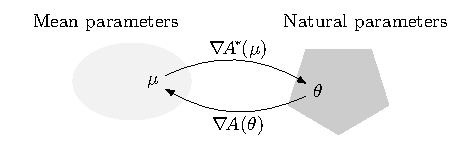
\includegraphics[width= .6\textwidth]{figs/duality} \\
	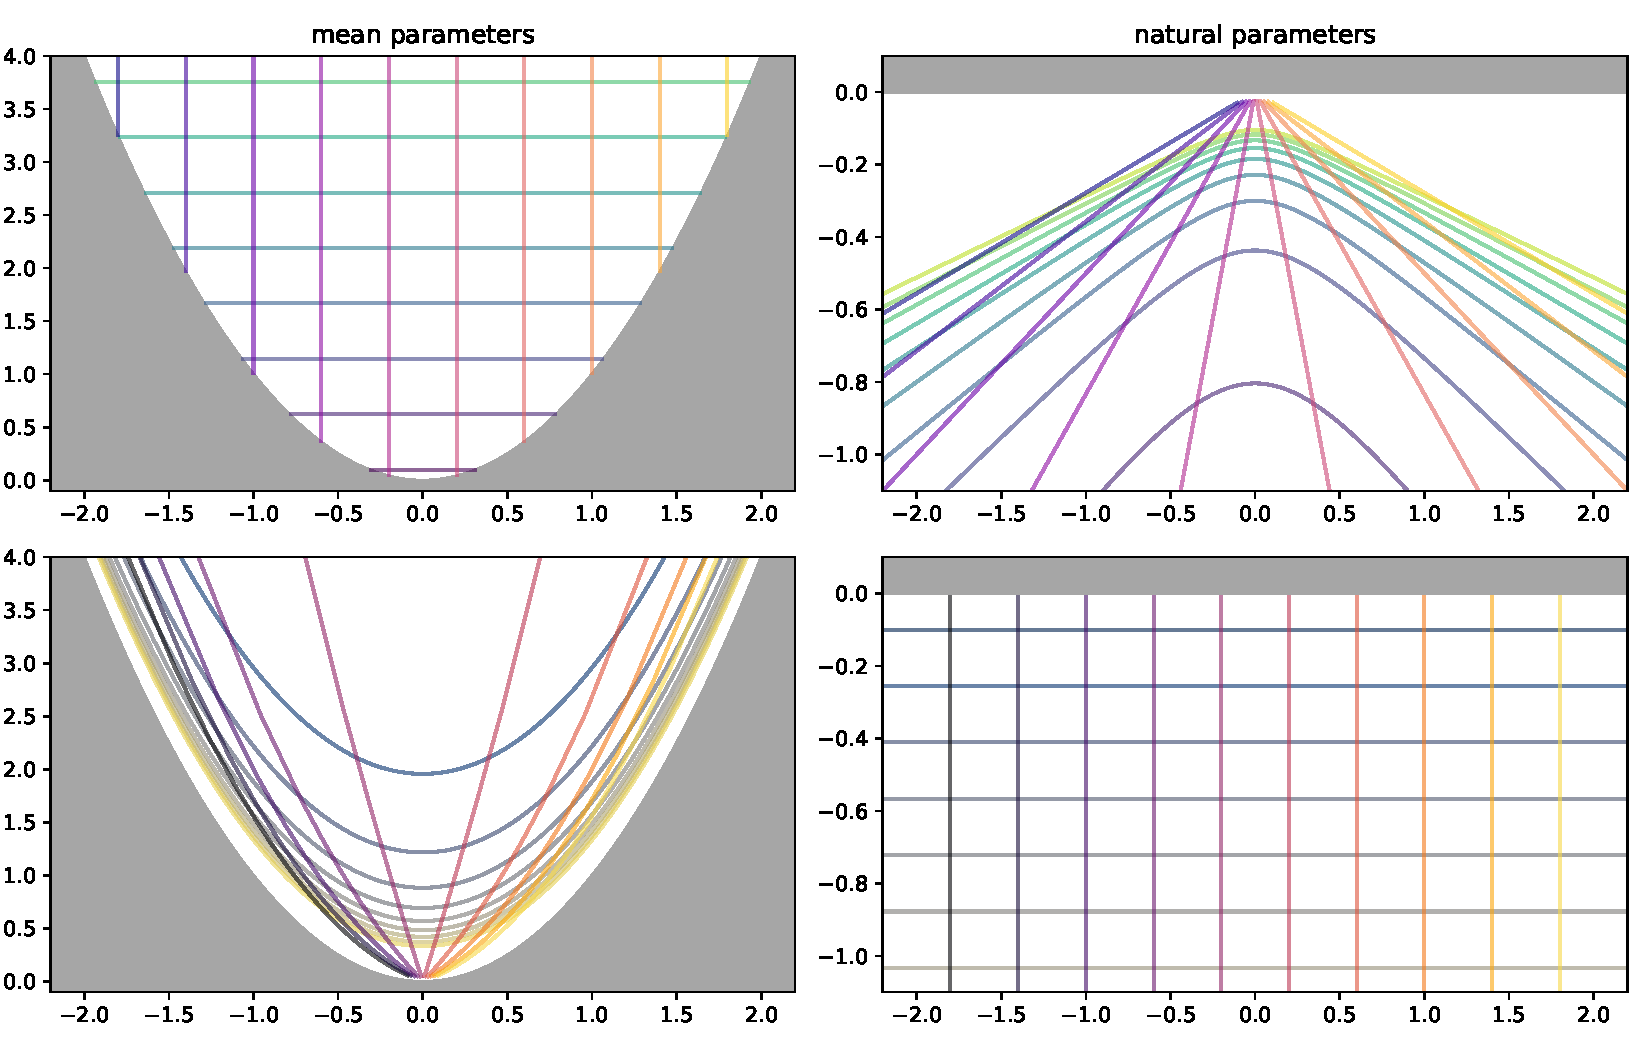
\includegraphics[width=.7\textwidth]{figs/2d/mirrormap.pdf}
	\caption{The gradient of the log-partition function and its dual, $(\nabla \logpart, \nabla \conj)$, form a bijection between the natural and mean parameters $\natp, \meanp$.Top figure reproduced from \citet{kunstner2020homeomorphic}. Bottom figure represents $\cN(\mu, \sigma^2)$.}
	\label{fig:duality}
\end{figure}
\begin{example}
For $\cN(0,\sigma^2)$,we can use the formula $\conj(\mu) = \mu \natp - \logpart(\natp)$ to get the entropy
\begin{align}
	\conj(\mu) = \half\left( -\log(\mu) + \log\frac{\pi}{2} - 1 \right) \; .
\end{align}
We can also take gradient and derivative of $\logpart(\natp)$ to retrieve the mean and covariance of the sufficient statistic $X^2$
\begin{align}
	\nabla\logpart(\natp) &= \frac{-1}{2 \natp} = \sigma^2 = \mu = \E[X^2] \\
	\nabla^2\logpart(\natp) &= \frac{1}{2 \natp^2} = 2 \sigma^4 = 2 \mu^2 = \Var(X^2) 
\end{align}
which we confirm thank to wikipedia since $\E[X^4] = 3 \sigma^4$ and thus $\Var(X^2) = \E[X^4] - \E[X^2]^2 = 3 \sigma^4 - \sigma^4 = 2 \sigma^4$.
\end{example}

\paragraph{Conjugate Prior}
One conjugate prior for $p(X|\natp)$ is
\begin{align}
    p(\natp) &\propto \exp( - n_0 \bregman(\natp ; \natp_0) )
\end{align}
where $n_0$ and $\natp_0$ are (hyper)parameters of the prior, and $\bregman(\natp ; \natp_0)$ is the Bregman divergence induced by $\logpart$ between $\natp$ and $\natp_0$
\begin{align}
    \bregman (\natp ; \natp_0)
    & = \logpart(\natp) - \logpart(\natp_0) 
    - \langle \nabla \logpart(\natp_0)  , \natp - \natp_0 \rangle
\end{align}
with $\nabla \logpart(\natp_0) = \expect[\natp_0]{T(X)} =: \meanp_0$ the mean parameter associated to $\natp_0$. 
Intuitively, $n_0$ is a number of fictive points observed from a distribution with parameter $\natp_0$.
We can re-write this prior as 
\begin{align}
    p(\natp) \propto 
    \exp( -n_0 \logpart (\natp) 
    + \langle n_0 \mu_0, \natp \rangle ) \; ,
\end{align}
which is the formula for the exponential family with sufficient statistics $(\natp ,\logpart(\natp))$ and with natural parameter $(n_0 \mu_0, -n_0)$.
The posterior given $\cD=(X_1,\dots, X_n)$ is then part of the same family, with natural parameters $(n_0 \mu_0 + \sum_i T(X_i) , -(n_0 + n))$.

\begin{example}
In the case of $\cN(0,\sigma^2)$, the logpartition function is $\logpart(\natp) = -\log(-\natp) /2 + \cst$, thus the conjugate prior is the exponential family with sufficient statistic $(\natp, \log(-\natp) )$, eg a negative \href{https://en.wikipedia.org/wiki/Gamma_distribution}{Gamma distribution}.
In particular,
\begin{align}
	p(\natp) 
	&\propto 
    \exp( -n_0 \logpart (\natp) 
    + \langle n_0 \mu_0, \natp \rangle ) \\
    &\propto \exp( \half[n_0] \log(-\natp) + n_0\mu_0 \natp ) \\
	&\propto (-\natp)^{1 + \half[n_0] -1 } e^{-n_0 \mu_0 (-\natp)} / Z
\end{align}
from which we infer the shape parameter $\alpha=1 + \half[n_0]$ and the rate parameter $\beta = n_0 \mu_0$, eg $\natp \sim \Gamma (1+\half[n_0] , n_0 \mu_0)$. After seeing $n$ samples, the posterior is $\Gamma\left(1+\half[n_0+n] , n_0 \mu_0 + \sum_i T(X_i) \right)$.
\end{example}

\paragraph{Maximum A Posteriori (MAP).}
The negative log-likelihood of the prior is
\begin{align*}
    -\log p(\natp) = n_0 (\logpart(\natp)  - \natp^\top \meanp_0 ) + \cst
\end{align*}
Thus the joint log-likelihood of $\cD =(X_1,\dots,X_n,\natp)$ is
\begin{align}
    -\log p(\cD|\natp)p(\natp) 
    = (n_0+n) \logpart (\natp) 
    - \theta^\top \left(n_0 \meanp_0 + \sum_{i=1}^n T(X_i) \right) + \cst \; .
\end{align}
Minimizing this expression over $\natp$ yields the Maximum A Posteriori estimate
\begin{align}
    \hat \natp = \argmin_\natp -\log p(\cD|\natp) + n_0 \bregman(\natp ; \natp_0)
\end{align}
such that the MAP is
\begin{align}
    \nabla \logpart(\hat \natp_\text{MAP}) = \hat \meanp_\text{MAP}
    = \frac{n_0 \meanp_0 + \sum_{i=1}^n T(X_i) }{n_0+n} \; .
\end{align}
When $n_0=0$ -- eg we observed zero samples from the prior -- we recover the Maximum Likelihood Estimate (MLE)
\begin{align}
	\hat \mu_\text{MLE} = \frac{\sum_{i=1}^n T(X_i)}{n}
\end{align}
The MLE and MAP estimates are statistics of the dataset $\cD$. Given a random dataset, we wish to bound their deviation from the optimum $\natp^*$ or $\meanp^*$.


\section{Open Problem}
For a well-specified model, the suboptimality on the population log-likelihood is exactly the KL between our current model and the true distribution
\begin{align}
    \expect[X\sim p(.|\natp^*)]{-\log p(X|\natp) + \log p(X|\natp^*) }
	= \KL( p(.|\natp^*) ; p(.|\natp)) \; .
\end{align}
For the exponential family, the KL is also the Bregman divergence induced by the log-partition function (with switched arguments)
\begin{align}
	\KL( p(.|\natp^*) ; p(.|\natp)) 
	= \bregman (\natp ; \natp^*)  \; .
\end{align}
There is a general relationship between Bregman divergences and convex conjugates (notice the argument switching)
\begin{align}
	\bregman (\natp ; \natp^*)
    = \logpart(\natp) - \langle \natp , \mu^* \rangle + \conj(\mu^*)
    = \bregmanconj ( \meanp^* ; \meanp)
\end{align}
so in the end the suboptimality is a divergence, which can either be seen as a KL between distributions, as a divergence between natural parameters, or as a divergence between mean parameters
\begin{align}
\boxed{
	\KL( p(.|\natp^*) ; p(.|\natp))
    = \bregman (\natp ; \natp^*)
    = \bregmanconj ( \meanp^* ; \meanp) \; .
}
\end{align}
\begin{important}
The question is: how does this quantity behave when $\natp$ is the maximum-likelihood or the MAP estimate ? Can we get bounds on the following quantities
\begin{align}
	\label{eq:bregmanMLE}
	\expect[X_i\sim \natp^*]{\bregmanconj \left (\E [T(X)] ;  \inv{n}  \smallsum_i T(X_i) \right )} \leq \ ? \; , \\
	\label{eq:bregmanMAP}
	\expect[X_i\sim \natp^*]{\bregmanconj \left (\E [T(X)] ; \frac{n_0 \mu_0 + \smallsum_i T(X_i)}{n_0+n} \right )} \leq \ ? \; ,
\end{align}
where the outer expectation is on the dataset $X_1, \dots, X_n$?
\end{important}

\paragraph{Remark.}
What we are looking for is really akin to concentration inequality, expressed with a Bregman divergence instead of a norm. A key difference though, is that the random variable $T(X)$ is connected to the metric $\logpart$. Indeed expressions~\eqref{eq:bregmanMLE} or~\eqref{eq:bregmanMAP} can be infinite for another choice of random variable. For instance, if we plug in $\conj(\mu)= -\log(\mu)$, which defines a divergence on positive numbers, and $T(X) \sim \cN(0,1)$ which can be negative.

\paragraph{Remark 2.}
The expectation of the MLE may be infinite, for instance with $\cN(0,\sigma^2)$ and $n\leq 2$. Instead of taking the expectation,  we might want to bound this quantity in high probability, without resorting to Markov inequality, but that is a difficult endeavor.

Below we review all the attempts we made on this problem.

\tableofcontents

\section{Gaussian Variance Example}

\begin{example}
	For $\cN(0,\sigma^2)$, both the entropy and the log-partition are roughly negative logarithm $z\mapsto - \log(z)$. Which yields the same shape of Bregman divergence, as visible below (all three lines are equal)
\begin{align}
	\KL( \sigma_*^2 ; \sigma_n^2 ) 
	&= \half \left ( \frac{\sigma_*^2}{ \sigma_n^2} - 1 - \log \frac{\sigma_*^2}{ \sigma_n^2} \right) \\
	\bregmanconj( \mu_*; \mu_n) 
	&= \half \left ( \frac{\mu_*}{ \mu_n} - 1 - \log  \frac{\mu_*}{ \mu_n} \right) \\
	\bregman( \natp_n; \natp_* ) 
	&=  \half \left ( \frac{ \natp_n}{\natp_*} - 1 - \log  \frac{ \natp_n}{\natp_*} \right) \; .
\end{align}
\end{example}
In other words, this divergence measures the discrepancy between the ratio $\frac{ \natp_n}{\natp_*} =  \frac{\mu_*}{ \mu_n}  $ and $1$ via the function $\phi$
\begin{align}
	\phi(z) := \half (z - 1 - \log(z)) \\
	\bregman( \natp_n; \natp_* )   = \phi(\frac{ \natp_n}{\natp_*}) =  \phi(\frac{\mu_*}{ \mu_n})
\end{align}
as illustrated in Figure~\ref{fig:phi}. We can get a non-transcendental upper bound thanks to the inequality
\begin{align}
	1 - \inv{z} \leq \log(z) 
	\label{eq:log_bound} 
	\implies \phi(z) \leq \half (z + \inv{z}) - 1 = \frac{(z-1)^2}{2 z} \; .
\end{align}


\begin{figure}[ht]
	\centering
	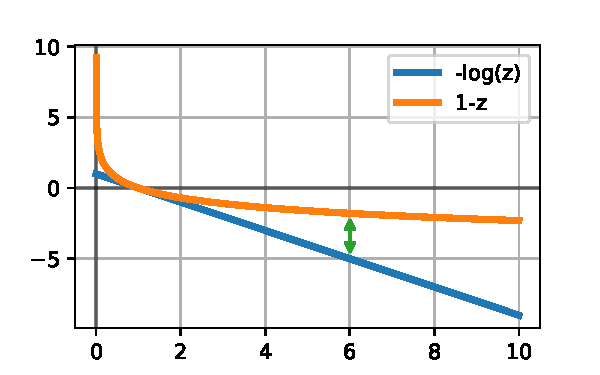
\includegraphics[width=.4\textwidth]{figs/bregmandef.pdf}
	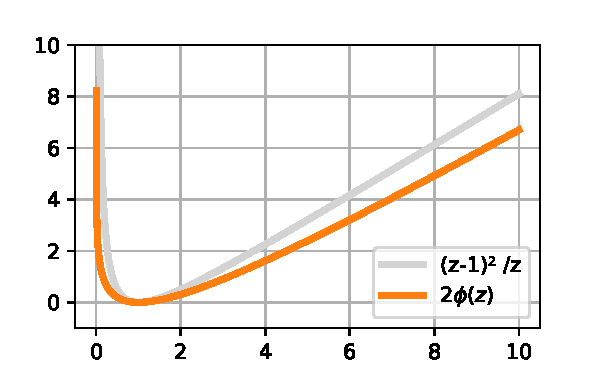
\includegraphics[width=.4\textwidth]{figs/phi.pdf}
	\caption{$\phi(z)$ is the Bregman divergence induced by $-\log(z)$. It is a barrier near $0$. As a result, it is poorly approximated by quadratics.}
	\label{fig:phi}
\end{figure}

\begin{figure}[ht]
	\centering
	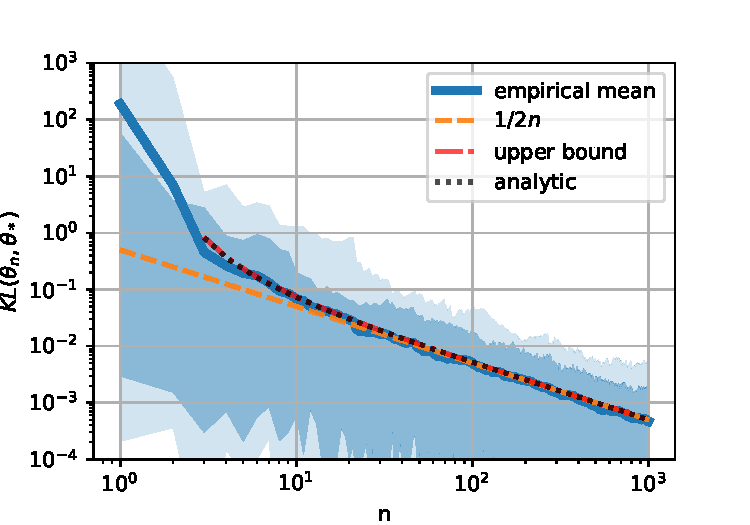
\includegraphics[width=.54\textwidth]{figs/asymptote.pdf}
	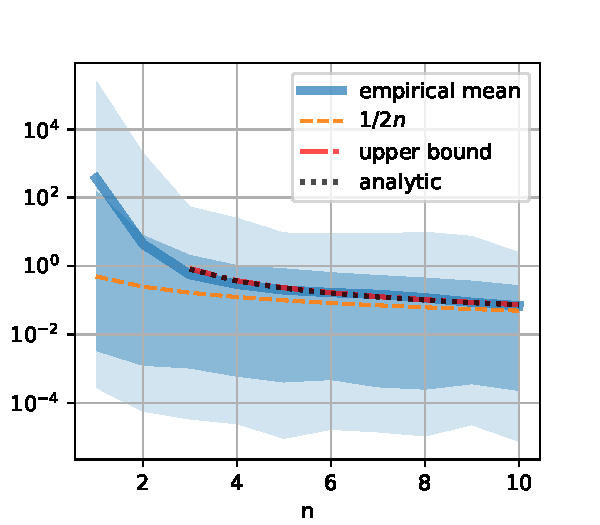
\includegraphics[width=.43\textwidth]{figs/fewsamples.pdf}
	\caption{Suboptimality of a Gaussian variance MLE against number of samples $n$. Bold curve is average over 100 trials,  dark shaded area is 90\% (dark) confidence interval, light shade is min-max interval.  
	\textbf{Left:} as $n$ increases, the suboptimality matches the $1/2N$ asymptote.
	\textbf{Right:} the first few samples significantly deviate from this behavior. In fact, for $n=1$ and $n=2$, the expected value is infinite, but we have a closed form solution and a simple upper-bound for $n>2$.
	}
	\label{fig:curves}
\end{figure}


\begin{example}
	\begin{theorem}[MLE Tight Bound]
	The MLE of $\cN(0,\mu_*)$ is $\hat \mu_n^\text{MLE} = \inv{n} \sum_i X_i^2 $.
	Its expected suboptimality is infinite when $n\leq 2$, and otherwise upper-bounded as
	\begin{align}
		 \expect{\bregmanconj( \mu_*; \hat \mu_n^\text{MLE}) }
			\leq \inv{2n} +\frac{2}{n(n-2)} \; .
			\label{eq:MLE_rate}
	\end{align}
\end{theorem}
\end{example}
This upper bound is asymptotically tight.
We illustrate its behavior against empirical data in Figure~\ref{fig:curves}.
 There is also a closed form for the multivariate generalization, thanks to the \href{https://en.wikipedia.org/wiki/Inverse-Wishart_distribution}{inverse Wishart distribution} and the \href{https://en.wikipedia.org/wiki/Wishart_distribution#Log-expectation}{expectation of the log-determinant of a Wishart}. The expected value is infinite whenever $n \leq d+1$ where $d$ is the dimension, and we report a similar upper bound in the appendix when $n>d+1$.
 
As for the MAP, we did not manage to get an asymptotically tight upper bound. Nevertheless, using inequality~\eqref{eq:log_bound}, we did get an interesting upper bound. 
To start, let us recall that the MAP of $\cN(0,\mu_*)$ is $\hat \mu_n = \frac{n_0 \mu_0 + \sum_i X_i^2}{n_0 + n}$.
Its expectation is simply $\mu_n= \frac{n_0 \mu_0 + n \mu^*}{n_0 + n}$.
We now present a lemma on its expected inverse.
\begin{lemma}[Expected MAP Natural Parameter]
	Let's define $a=n_0 \frac {\mu_0 }{ \mu^* }$. For any $n\geq 1$, the expectation of the natural parameter of the MAP of $\cN(0,\mu_*)$ is bounded as
	\begin{equation}
		\frac{\mu^*}{\mu_n}
		\leq \expect{\frac{\mu^*}{\MAPm}} 
		= \expect{\frac{\MAPt}{\natp^*}} 
		\leq \frac{n_0 +n}{a+ (n-2)_+}
		\label{eq:theta_expectation_bound}
	\end{equation}
	where $(x)_+ = \max(0,x)$.
\end{lemma}
Note that the lower bound is a simple consequence of the convexity of the inverse function. 
Using this lemma, along with the log upper bound on the logarithm~\eqref{eq:log_bound}, we get a convergence rate for the MAP. 
\begin{example}
\begin{theorem}[MAP Bound]
 Let us  define
 \begin{align}
	b = \frac{(1 + \inv{n_0} - \frac{\mu_0}{\mu^*})^2}{2 (\frac{\mu_0}{\mu^*}+\frac{(n-2)_+}{n_0})(1 + \frac{n}{n_0} )} \; .
 \end{align}
The expected suboptimality of the MAP of $\cN(0,\mu^*)$ with prior hyper-parameters $(n_0,\mu_0)$ is
 \begin{equation}
	\expect{\bregmanconj( \mu_*; \hat \mu_n^\text{MAP})}
	\leq \begin{cases}
		\inv{2(n_0+1)}  +  b\ \text{if}\ n=1,\\
		\frac{1}{n_0 \frac{\mu_0}{\mu^*} +n-2} + b \ \text{if}\ n\geq 2
	\end{cases}
	\label{eq:MAP_rate}
\end{equation}
\end{theorem}
\end{example}
This inequality highlights a clear variance-bias decomposition.
In particular, there is no bias term when $\frac{\mu_0}{\mu^*} =1 + \inv{n_0} $, which happens when the prior is slightly larger than the ground truth.  For instance, when $n_0=1$, it encourages us to set $\mu_0 = 2 \mu^*$.
Remark that the variance term is not asymptotically tight as the log-inequality we used \eqref{eq:log_bound} is not quadratically tight around $1$. We are basically losing a factor 2 compared to $1/2n$.

Using the same bound on the log~\eqref{eq:log_bound}, we  get a loose bound on the MLE, which is useful for comparison purposes.
We relate these loose convergence rates of MAP and MLE in Figure~\ref{fig:MAP_rate}.
\begin{example}
\begin{corollary}[MLE Loose Bound] When $n\geq 2$, the MLE expected loss is upper bounded as
\begin{equation}
	\expect{\bregmanconj( \mu_*; \hat \mu_n^\text{MLE}) }
	\leq \inv{n-2} \; .
	\label{eq:MLE_loose_rate}
\end{equation}
\end{corollary}
\end{example}


\begin{figure}[ht]
	\centering
	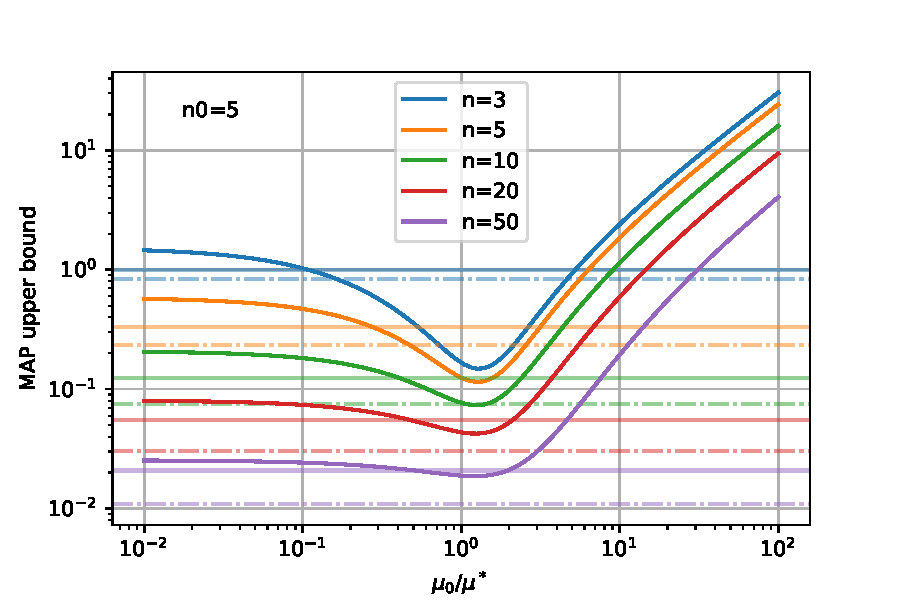
\includegraphics[width=.7\textwidth]{figs/MAP_rates/MAP_rate_n0=5.pdf}
	\caption{
	Convergence rate of MAP~\eqref{eq:MAP_rate} 
	\label{fig:MAP_rate} against the ratio between initialization and optimum $ \frac{\mu_0}{\mu^*}$. 
	We also report the tight convergence rate of MLE~\eqref{eq:MLE_rate} (dash-dotted horizontal lines), and the loose upper bound~\eqref{eq:MLE_loose_rate} (horizontal lines). 
	We report these curves for various values of $n$, and $n_0=5$. 
	We observe that the rate of MAP is significantly better (lower) than the rate of MLE, only when we guessed $\mu_0$ right, within an order of magnitude from $\mu^*$, and for a small number of sample ($n<10$). 
	This observation hints towards the optimality of MLE for large $n$. 
	It makes me feel very interested in convergence rates of MAP in the overparametrized regime $n<\dim(T(X))$.
	}
\end{figure}

\section{Euclidean Behaviour}
Often we can relate this Bregman suboptimality with the $\ell^2$ distance in mean parameter space. 
\TODO{Add base measure to add here a discussion of the euclidean case -- the mean of a gaussian}
\paragraph{If $\conj$ is $L$-Lipschitz} (e.g. $\logpart$ is defined within the $\ell^2$-ball of radius $L$), then
\begin{align}
    \bregmanconj(\mu^* ; \mu) 
    \leq L \norm{\mu^* - \mu} + \norm{\natp} \norm{\mu^* - \mu}
    \leq 2L \norm{\mu^* - \mu}
\end{align}
so $\bregmanconj$ is $2L$-Lipschitz.
Since the empirical average converges in expectation to the population mean at a rate of $1/\sqrt{n}$ in $\ell^2$ norm, we know that this bound applies to the log-likelihood.
\paragraph{If $\conj$ is $L$-smooth} (e.g. $\logpart$ is $L^{-1}$-strongly convex), then
\begin{align}
    \bregmanconj(\mu^* ; \mu) 
    \leq \frac{L}{2} \norm{\mu^* - \mu}^2
\end{align}
so $\bregmanconj$ is upper bounded by a quadratic. In expectation, it should converge at a rate $1/n$.

\paragraph{$\ell^2$-norm Analysis}
Let us make these statements more precise. A bound on the variance becomes a bound on the variance of the average
\begin{align}
	\Var T(X) = \E \norm{T(X) - \mu^*}^2 = \sigma^2 \\
	\implies \E \norm{\mu^* -  \inv{n}  \smallsum_i T(x_i)}^2 = \frac{\sigma^2}{n} 
\end{align}
eg the variance of the mean is $n$ times smaller than the variance of the samples.
Adding a reference mean $\mu_0$ to get the MAP yields
\begin{align}
	\E \norm{\mu^* -  \frac{n_0 \mu_0 + \smallsum_i T(x_i)}{n_0+n} }^2 
	&= \frac{n}{(n+n_0)^2} \sigma^2 +  \frac{n_0^2}{(n+n_0)^2} \norm{\mu^* -  \mu_0}^2 \\
	&= O\left(\frac{\sigma^2}{n} \right) + O\left(\frac{\norm{\mu^* -  \mu_0}^2}{n^2} \right)
\end{align}
so we have a variance term in $O(n^{-1})$ and a bias term decreasing as $O(n^{-2})$. Let's see if we can get similar estimates for arbitrary exponential families !

\section{Asymptotic Behaviour}
In the limit, the MAP estimates reach a rate $O(1/2n)$. This is shown by approximating the Bregman divergence using a second order Taylor expansion
\begin{align}
    \bregmanconj(\mu^* ; \mu) 
    &= \half (\mu - \mu^*)^\top \nabla^2\conj(\mu^*)(\mu - \mu^*)  
    + O(\norm{\mu - \mu^*}^3)\\
    &=\half  \norm{\mu^* - \mu}^2_{\nabla^2\conj(\mu^*)}
    + O(\norm{\mu - \mu^*}^3)
\end{align}
where we introduced the Mahalanobis distance induced by the matrix 
\begin{align}
    \nabla^2\conj(\mu^*) 
    = \nabla^2\logpart(\natp^*)^{-1} 
    = \Cov_{\natp^*}[T(X)]^{-1} 
    =: \mSigma^{-1}  \; .
\end{align}
To exploit this approximation, let us extend the $\ell^2$ norm results to a Mahalanobis distance induced by matrix $\mM$
\begin{align}
	\E \half \norm{\mu^* -  \inv{n}  \smallsum_i T(x_i)}_\mM^2 = \inv{2 n} \Tr(\mM \mSigma)
\end{align}
where $\mSigma$ is the covariance of $T(X)$. We retrieve $\nicefrac{\sigma^2}{n}$, the variance divided by the number of samples, when the metric is the identity $\mM=\mI$.  For the MLE we get
\begin{align}
	\E \bregmanconj \left (\E [T(X)] ;  \inv{n}  \smallsum_i T(X_i) \right ) = \frac{d}{2n} + O(n^{- \frac{3}{2}})
\end{align}
and for the MAP we  get 
\begin{align}
	\E \half \norm{\mu^* -  \frac{n_0 \mu_0 + \smallsum_i T(x_i)}{n_0+n} }^2_{\mSigma^{-1}}
	&= \frac{n d}{2(n+n_0)^2}  +  \frac{n_0^2}{(n+n_0)^2} \half \norm{\mu^* -  \mu_0}^2_{\mSigma^{-1}} \\
	&= \frac{d}{2n} + O\left(\frac{1 + \norm{\mu^* -  \mu_0}^2_{\mSigma^{-1}} }{n^2} \right) \; .
\end{align}
or 
\begin{align}
\label{eq:MAP_asymptote}
	\E \bregmanconj \left (\E [T(X)] ;  \frac{n_0 \mu_0 + \smallsum_i T(x_i)}{n_0+n} \right ) 
	= \frac{d}{2n} + O(n^{- \frac{3}{2}})
\end{align}
Remark how the variance does not even appear, only the dimension divided by $n$ really matters. I find this result quite spectacular : the convergence speed of MLE is not affected by the covariance of sufficient statistics, and for MAP it matters only in the $O(n^{-2})$ term.
Indeed this is because it is hidden within the Bregman divergence loss. 
Anyway that's all good for asymptotic results, but we are interested in a finite sample analysis. How do we get this ?

\section{Bias-Variance Decomposition}
\newcommand{\bias}[1]{\textcolor{Red}{\underbrace{\textcolor{black}{#1}}_{\text{bias}}}}
\newcommand{\variance}[1]{\textcolor{Green}{\underbrace{\textcolor{black}{#1}}_{\text{variance}}}}

\subsection{Dual Expectation Pivot.}
Let $\hat \mu_n = \frac{n_0 \mu_0 + \sum_i T(X_i)}{n_0 + n}$ be the MAP estimate of the mean (dual) parameter, $\hat \natp_n = \nabla \conj(\hat \mu_n)$ the corresponding natural (primal) parameter, and
$\mu_n = \expect{\hat \mu_n} = \frac{n_0 \mu_0 + n \mu^*}{n_0 + n}$ the expected MAP dual estimate
Taking $\mu_n$ as a pivot, we can decompose the expected suboptimality in 3 terms -- e.g. 
\begin{align}
	\expect{\bregmanconj(\mu^* ; \hat \mu_n)} 
	&= \conj(\mu^* ) 
	\pm \conj(\mu_n)
	-  \expect{\conj(\hat \mu_n)}
	+ \E[\langle \hat \natp_n ; \hat \mu_n   \pm \mu_n - \mu^*  \rangle ] 
	\nonumber \\
	&= \conj(\mu^* ) 
	- \conj(\mu_n)  + \E[\bregmanconj(\mu_n, \MAPm)]
	+ \langle \E[\hat \natp_n] \pm \nabla \conj(\mu_n) ;  \mu_n - \mu^* \rangle
	\nonumber\\
	& = \bias{\bregmanconj(\mu^*; \mu_n)}
	+ \frac{n_0}{n+n_0} \langle  \bias{\mu_0 - \mu_*} ; \variance{\E[\hat \natp_n] - \natp_n} \rangle 
	+ \variance{\E[\bregmanconj(\mu_n, \MAPm)]} \; .
	\label{eq:bias-mixed-variance}
\end{align}
Remark that unless $\conj$ is $\ell^2$, or unless we are in a degenerate case with $\hat \mu_n$ a Dirac, the dual and primal expectation represent different distributions $\theta_n \neq \expect{\hat \theta_n}$, which is why the mixed term (bias-variance scalar product) is non-zero.
Asymptotically, these terms behave like : bias $O(n^{-2}$, mixed $O(n^{-3})$ and variance $O(n^{-1})$, but the story is different for finite samples.
We know for sure that the bias and the variance term are positive, but the mixed bias-variance term may be negative, which removes some appeal of this decomposition. 
Fortunately there is another decomposition revolving around the primal expectation.

%\begin{figure}[ht]
%	\centering
%	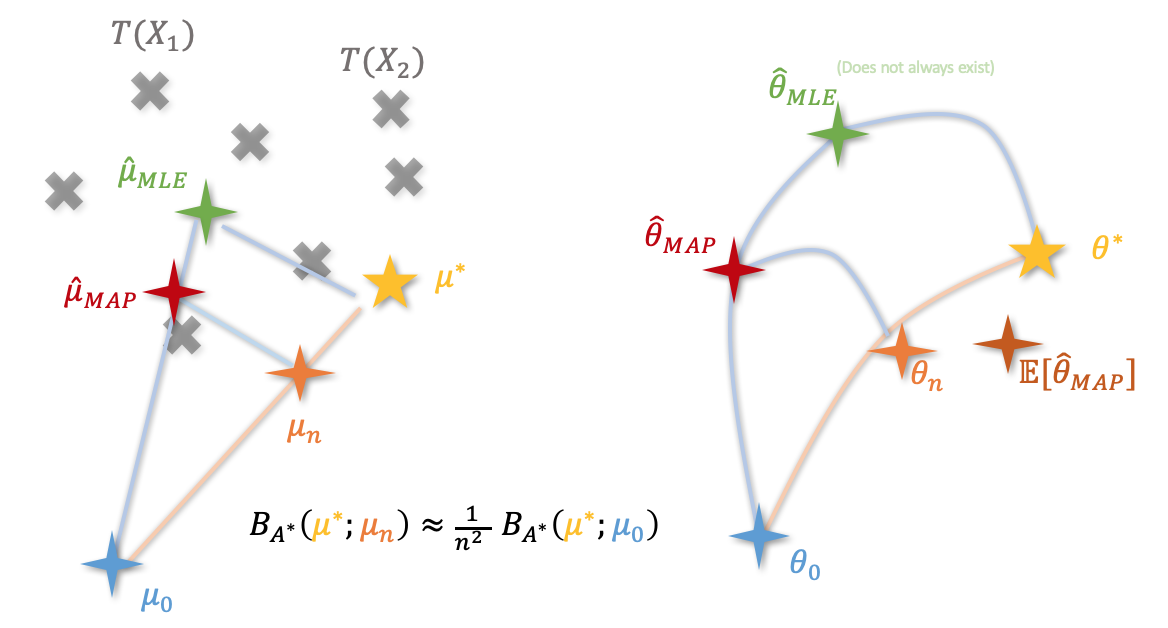
\includegraphics[width=.8\textwidth]{figs/bias-variance.png}
%	\caption{A schematic illustration of the different characters featured in the bias-variance decomposition.}
%	\label{fig:bias-variance}
%\end{figure}

\begin{figure}[ht]
	\centering
	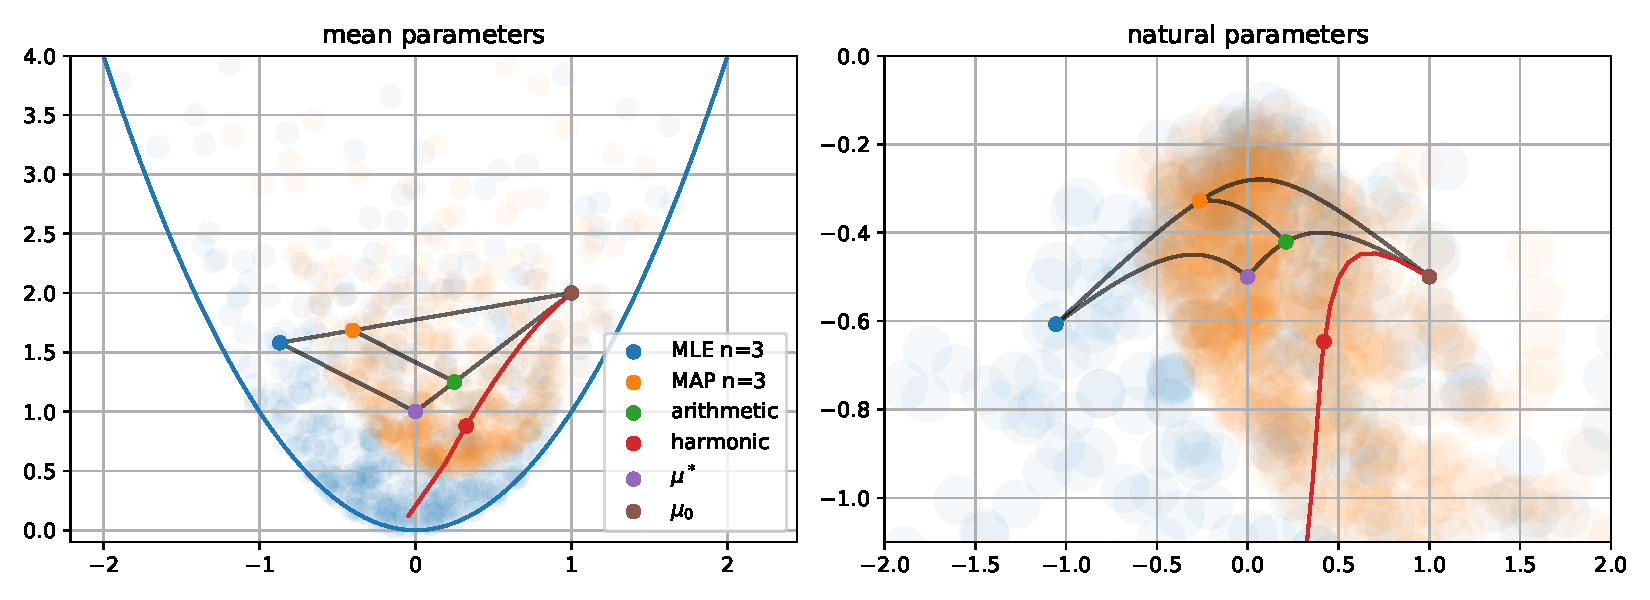
\includegraphics[width=\textwidth]{figs/thales/numerical_schema_n=3.pdf}
	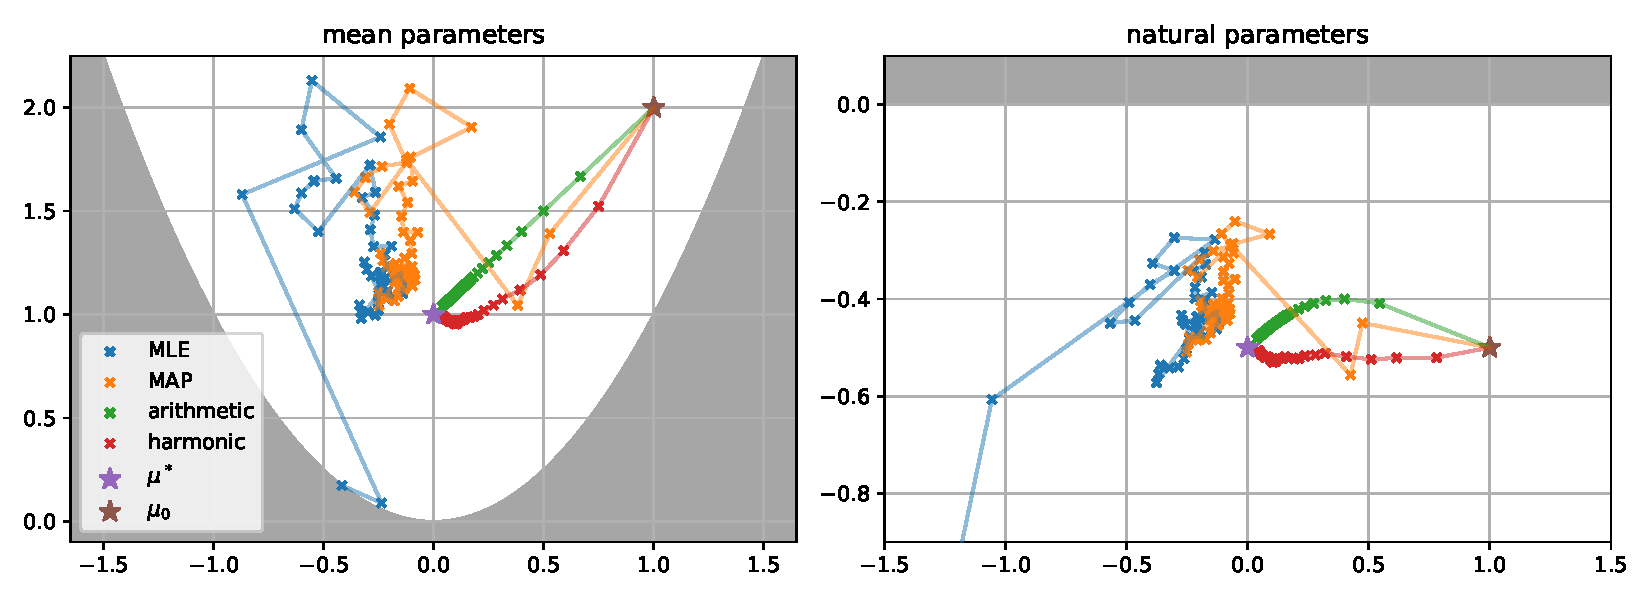
\includegraphics[width=\textwidth]{figs/2d/gaussian_convergence.pdf}
	\caption{A numerical illustration of the different characters featured in the bias-variance decomposition, for a 1D Gaussian $\cN(\mu, \sigma^2)$, for 1 time step  and many repetitions with $n=3$ (top) illustrating the effect of $n_0$ with the Thales triangle. Or $50$ time-steps at once and 1 repetition (bottom), illustrating the convergence behavior.}
	\label{fig:bias-variance-numerical}
\end{figure}


\subsection{Primal Expectation Pivot}
Let $\tilde \theta_n := \expect{\hat \theta_n}$ and $\tilde \mu_n = \nabla \logpart(\tilde \theta_n )$ be the primal and dual parameters of the primal expectation of the MAP.
As described by \citet[Theorem 0.1]{pfau2013generalized}, the  expected Bregman decomposes like
\begin{align}
	\expect{\bregmanconj(\mu^* ; \hat \mu_n)} 
	&= \bias{\bregmanconj(\mu^* ; \tilde \mu_n)}
	+ \variance{\expect{\bregmanconj(\tilde \mu_n ; \MAPm)}} \\
	\expect{\bregman(\MAPt; \natp^*)} 
	&= \bias{\bregman(\E[\MAPt]; \natp^*)}
	+ \variance{\expect{\bregman(\MAPt; \E[\MAPt])}}  \; .
	\label{eq:primal_pivot}
\end{align}

\paragraph{Illustrations.}
We show these decompositions for $\cN(0,\sigma^2)$ in Figure~\ref{fig:variance_decomposition} and  $\cN(\mu, \sigma^2)$ in Figure~\ref{fig:gaussian_decomposition}.
In particular for $\cN(\mu, \sigma^2)$, we illustrate the characters featured in both of these decompositions $\hat \mu_n^\text{MLE},\hat \mu_n^\text{MAP},\mu_n,\tilde \mu_n, \mu^*$ and $\mu_0$ (and corresponding primal parameters)  in Figure~\ref{fig:bias-variance-numerical}.

\begin{figure}[ht]
	\centering
	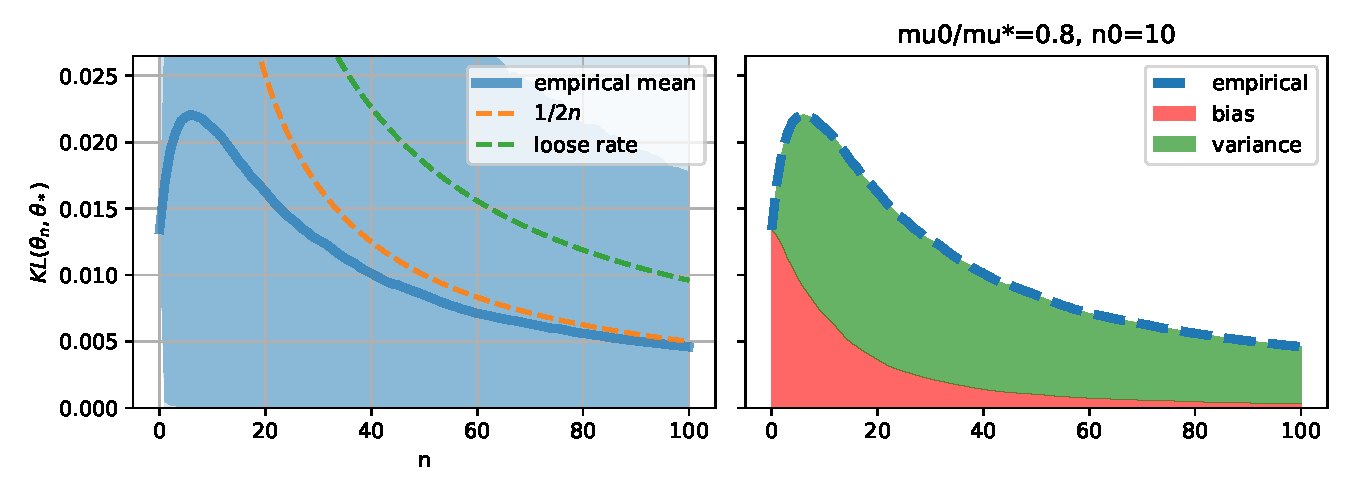
\includegraphics[width=\textwidth]{{figs/biasvariance/linear_ratio=0.8_n0=10}.pdf}
	\caption{
	\textbf{Gaussian variance $\cN(0,\sigma^2)$ example. Left:} training curves and analytic upper bound. 
	\textbf{Center:} bias-mixed-variance decomposition, using the arithmetic mean.
	\textbf{Right:} bias-variance decomposition, using the harmonic mean.
	}
	\label{fig:variance_decomposition}
\end{figure}

\begin{figure}[ht]
	\centering
	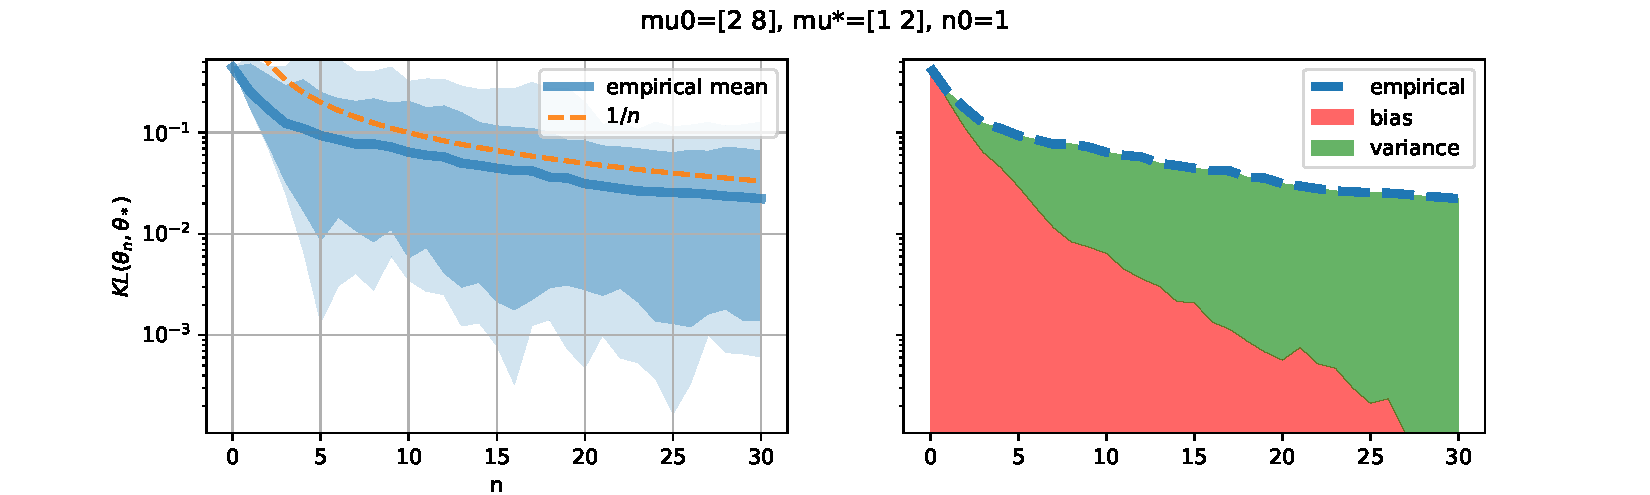
\includegraphics[width=\textwidth]{{figs/gaussians/log_n0=1}.pdf}
	\caption{
	\textbf{Full gaussian $\cN(\mu, \sigma^2)$ example. Left:} training curves and analytic upper bound. 
	\textbf{Center:} bias-mixed-variance decomposition, using the arithmetic mean.
	\textbf{Right:} bias-variance decomposition, using the generalized mean.
	}
	\label{fig:gaussian_decomposition}
\end{figure}

\subsection{About Variance and Covariance}

\begin{lemma}
\label{lem:covariance}
Taking  $\MAPt$ and $\MAPm$ as the primal and dual parameters of the MAP estimate, and $\tilde \mu_n$ the primal expectation and $\mu_n$ the dual expectation, the following identities hold
	\begin{align}
	\Cov(\hat \natp_n ; \MAPm )  
	&=\expect{\bregmanconj(\MAPm ; \mu_n)
	+ \bregmanconj(\mu_n ; \MAPm)} \\
	&=\expect{\bregmanconj(\MAPm ; \tilde \mu_n)
	+ \bregmanconj(\tilde \mu_n ; \MAPm)} \; .
\end{align}
\end{lemma}
\begin{proof}
By the three point identity (or plain derivation), we have 
\begin{align}
	\bregmanconj(\MAPm ; \mu_n)
	+ \bregmanconj(\mu_n ; \MAPm)
	= \langle \nabla \conj (\hat \mu_n) - \nabla \conj(\mu_n) ;  \hat \mu_n - \mu_n \rangle 
	= \langle \MAPt - \theta_n;  \MAPm- \mu_n \rangle 
\end{align}
Taking the expectation,  the constant $\theta_n$ disappears since $\expect{\hat \mu_n - \mu_n}=0$.
\begin{align}
	\expect{\langle \MAPt - \theta_n;  \MAPm- \mu_n \rangle } 
	 = \expect{\langle \MAPt; \MAPm \rangle} - \langle \expect{\MAPt} ; \MAPm \rangle
	= \Cov(\hat \natp_n ; \hat \mu_n ) 
\end{align}
which is the first identity. We get the second identity by symmetry between the primal and the dual.
\end{proof}

Note that, as a corollary, the covariance between primal and dual MAP
$\Cov(\hat \natp_n ; \hat \mu_n )$ is positive, and it can be seen as a non-linear variance of $\hat \mu_n$ -- e.g. we can define a variance operator with a non-linear monotone operator $\nabla\conj$ plugged in the middle $\Var_{\nabla \conj}(\hat \mu_n) := \Cov(\nabla\conj(\hat \mu_n) ; \hat \mu_n ) \geq 0$.

\paragraph{Expansion}
We can expand  $\hat \mu_n - \mu_n$ to get another formulation of this covariance
\begin{align}
	\expect{\langle \hat \natp_n ; \hat \mu_n - \mu_n \rangle}
	&= \expect{\langle \hat \natp_n ; \frac{\sum_i T(X_i) - \mu^*}{n+n_0} \rangle}  \\
	& = \frac{n}{n+n_0} \expect{\langle \hat \natp_n ; T(X_0) - \mu^*\rangle} \\
	&= \frac{n}{n+n_0} \Cov(\hat \natp_n ; T(X_0) ) 
	\label{eq:covariance_expansion}
\end{align}
where we used the property that all data points play a symmetric role to remove the sum over $i$.

\subsection{Triangle Scaling Exponents}

\citet{hanzely2021accelerated} 
defines the Triangle Scaling Exponent, to characterize an acceleration Bregman methods. The exponent $\gamma$ of a Bregman divergence $\cB$ is defined as the largest coefficient such that $
	\forall x_0, x_1, x_2, \forall \lambda\in[0,1],$
\begin{align}
	\cB((1-\lambda)x_0 + \lambda x_1 ; (1-\lambda)x_0 + \lambda x_2)
	\leq \lambda^\gamma \cB(x_1 ; x_2) \; .
\end{align}
Geometrically, for any triangle, it tells us a shape within which the geodesic triangle is contained (to clarify with a picture.)
It is related to Thales triangle.
We precisely have a Thales triangle with the dual expectation pivot, meaning we can relate the MAP variance term with the MLE expected suboptimality. Writing $\lambda = \frac{n}{n+n_0}$, we observe
\begin{align}
	\MAPm^\text{MAP} &= (1-\lambda)\mu_0 + \lambda \MAPm^\text{MLE} \\
	\mu_n &= (1-\lambda)\mu_0 + \lambda \mu^*
\end{align}
thus
\begin{align}
	\expect{\bregmanconj(\mu_n; \MAPm^\text{MAP})}
	\leq \left (\frac{n}{n+n_0} \right)^\gamma \expect{\bregmanconj(\mu^*; \MAPm^\text{MLE})} \; .
\end{align}
This relationship between the MAP variance and the MLE may be void, as the MLE expected loss may be infinite. But in some settings it might be helpful to characterize the MAP convergence.
For instance, this same paper says that for a gaussian variance, $\gamma=1$. Then they proceed to define an intrinsic scaling exponent, with a local scaling factor. This intrinsic exponent is always 2 for Bregman divergences induced by a convex and $\cC^2$ function. They use this fact to derive an accelerated algorithm.

\clearpage

\section{Optimization Perspective}
\paragraph{Problem.}
We want  to solve the following problem
\begin{align}
	f^* = \min_\natp \E[f(\natp ; X)] := -\langle \E[T(X)] ; \natp \rangle + \logpart(\natp)
\end{align}
where $\logpart$ is a convex function.
We assume access to stochastic oracles $X \sim p(X | \natp^*)$ -- e.g. we observe $X$ such that $\E[T(X)] = \mu^*$ and we can compute  stochastic function values and gradients 
\begin{align}
	f(\natp ; X) &= -\langle T(X) ; \natp \rangle + \logpart(\natp) \\
	\nabla f(\natp ; X) &= \nabla \logpart(\natp) - T(X)\; .
\end{align}
It is important to note that our problem is merely a stochastic linear tilt of the convex function $\logpart$, yet none of the convergence rates we studied applied to this setting.

\paragraph{Algorithms.}
We observe $n$ data points $X_i$. 
We are studying two algorithms solving this problem : MLE and MAP.
\begin{align}
	\MAPm^\text{MLE} &= \inv{n}\sum_{i=1}^n T(X_i) 
	&\MAPt^\text{MLE} &= \nabla\logpart^{-1}(\MAPm^\text{MLE}) \\
	\MAPm^\text{MAP} &= \frac{n_0\mu_0 + \smallsum_{i=1}^n T(X_i)}{n_0 + n}
	&\MAPt^\text{MAP} &= \nabla\logpart^{-1}(\MAPm^\text{MAP})	
\end{align}

\paragraph{Interpretation.}
As we will see in the two upcoming sections, MAP can be seen as an application of more generic iterative algorithms with divergence $\bregman$ and initialization $\natp_0$ : 
\begin{itemize}
	\item Stochastic Bregman Proximal Point with learning rate $\inv{n_0+n}$,
	\item Stochastic Mirror Descent with learning rate  $\inv{n_0+n +1}$.
\end{itemize}
In both cases, $f(\natp)$ is convex and 1-smooth  and 1-strongly convex relative to the potential $\logpart$. Be cautious that the learning rate is decreasing.

\paragraph{Goal.} We want to bound the suboptimality $f(\natp) - f^*$ as a function of the number of samples. 

\section{Stochastic Bregman Proximal Point}
\subsection{Correspondence with MAP}
For a dataset of independent samples $\cD_n = \{X_1,\dots,X_n\}$, the posterior can be seen iteratively
\begin{align}
	p(\natp |\cD_n)
	=p(\natp|X_n,\cD_{n-1})
	\propto p(X_n|\natp,\cD_{n-1}) p(\natp|\cD_{n-1})
	=p(X_n|\natp)p(\natp |\cD_{n-1}) \; .
\end{align}
For the MAP of the exponential family with a Bregman conjugate prior, the posterior takes the form
\begin{align}
	- \log p(\natp | \cD_n) 
	&= \sum_{i=1}^n -\log p(X_i | \natp) - \log p(\natp) + \cst\\
	&= \sum_i - \langle T(X_i) ; \natp \rangle  + n \logpart(\natp) + n_0 \bregman(\natp ; \natp_0) +\cst \\
	&= (n+n_0)\logpart(\natp)  - \langle n_0 \mu_0 + \sum_i T(X_i) ; \natp \rangle + \cst \\
	&= (n+n_0) \bregman(\natp; \hat \natp_n^\text{MAP}) + \cst \; ,
\end{align}
so we immediately get the recursion
\begin{align}
    \hat \natp_n^\text{MAP}
    &= \argmin_\natp - \log p(\natp | \cD_n) \\
    &= \argmin_\natp - \log p(X_n|\natp) - \log p(\natp | \cD_{n-1}) \\
    &= \argmin_\natp f(\natp; X_{n}) + (n+n_0) \bregman(\natp; \hat \natp_{n-1}^\text{MAP})  \; .
    \label{eq:SBPP}
\end{align} 
Coincidentally, this is exactly the formula of a Stochastic Bregman Proximal Point update on the function $f(\natp) = \E_X[-\log p(X|\natp)]$ , with step-size $\lr_n = \inv{n+n_0}$. As a reminder this algorithm is defined with the update
\begin{align}
	 \hat \natp_n
    &= \argmin_\natp \lr_n f(\natp; X_{n}) + \bregman(\natp; \hat \natp_{n-1}) \\
    \iff \nabla \logpart(\natp_{n-1}) &= \nabla\logpart(\natp_n) + \lr_t \nabla f(\natp_n ; X_t) \; .
\end{align}
In words, if it converges to $\natp^*$, it can be seen as a backward mirror ascent starting from $\natp^*$.

\subsection{Straightforward Analysis}

\subsubsection{Deterministic Bregman Proximal Point}
Deterministic Bregman proximal point. was first published in \citet{eckstein1993nonlinear} with an asymptotic convergence property, soon completed by a finite sample convergence rate in \citet{chen1993convergence}. 
This convergence rate relies on the three points lemma (Appendix~\ref{app:3points})
\begin{align}
	 \forall \natp, \lr_t f(\natp) + \cB(\natp ; \natp_t) \geq \lr_t f(\natp_{t+1}) + \cB( \natp; \natp_{t+1}) +\cB(\natp_{t+1} ; \natp_{t}) \; .
\end{align}

\paragraph{Monotonicity of Function Values.}
Applying it with $\natp=\natp_t$, we prove that function values are decreasing
\begin{align}
	f(\natp_{t+1})  \leq f(\natp_{t})  - \inv{\lr_t} \underbrace{\left (\cB(\natp_{t+1} ; \natp_{t}) + \cB(\natp_{t} ; \natp_{t+1}) \right) }_{=: \cS(\natp_{t} ; \natp_{t+1})}
\end{align}
where we introduced $\cS$ the symmetrized Bregman divergence
\begin{align}
	\cS(x; y) = \cB(x ; y) + \cB(y ; x) = \langle\nabla A(x) - \nabla A(y) ; x-y \rangle \; .
\end{align}

\paragraph{Descent Lemma and Telescopic Sum.}
Applying the three point lemma with $\natp=\natp^*$ (assuming such a minimizer exists), we obtain a telescopic sum
\begin{align}
	\lr_t(f(\natp_{t+1}) - f(\natp^*)) +  \cB(\natp_{t+1} ; \natp_{t}) 
	&\leq  \cB( \natp^*; \natp_{t})  - \cB( \natp^*; \natp_{t+1}) \\
	\implies \sum_{t=0}^{T-1} \lr_t (f(\natp_{t+1}) - f(\natp^*)) 
	+ \sum_{t=0}^{T-1} \cB(\natp_{t+1} ; \natp_{t}) 
	&\leq \cB( \natp^*; \natp_{0})  - \cB( \natp^*; \natp_{T})  
	\leq \cB( \natp^*; \natp_{0})  \; ,
\end{align}
which proves on the way that the total path length $ \sum_{t=0}^{t-1} \cB(\natp_{t+1} ; \natp_{t}) $ is bounded.
Using the monotonicity of $f(\natp_t)$, we get
\begin{align}
	f(\natp_{T}) - f(\natp^*) \leq \frac{\cB( \natp^*; \natp_{0}) }{\sum_{t=0}^{T-1} \lr_t} \; .
\end{align}
This upper bound converges to $0$ whenever the sum of step-sizes converges to $0$. 
This rate can be arbitrarily fast because the oracle is strong. Indeed, taking an inifinite step-size solves the problem with one iteration, but the update is (theoretically) harder to solve for larger step-sizes.

\subsubsection{Stochastic Bregman Proximal Point.}
While \citet{eckstein1998approximate} shows some asymptotic convergence of the Bregman proximal point algorithm when each iteration is only solved approximately, we are not aware of published analysis when iterations are stochastic.

\paragraph{Variance Assumption.}
The deterministic proof does not transpose immediately to the stochastic setting.
We need an assumption on the quality of the stochastic estimates $f(. ; x)$. 
As we will see soon, the most straightforward such assumption is 
\begin{align}
\boxed{\expect{f(\natp_{t+1}) - f(\natp_{t+1} ; X_{t+1})} \leq \lr_t \sigma^2 \; , }
\label{eq:proximal_variance}
\end{align}
e.g. we relate the stochastic function value on the next iterate to the function value.
Asymptotically, this assumption is equivalent to the one of~\citet{hanzely2018fastest}. 
To see this, linearize $f(\natp_{t+1})$ and $f(\natp_{t+1} ; X_{t+1}) $ in $\natp_t$
\begin{align}
	\expect{f(\natp_{t+1}) - f(\natp_{t+1} ; X_{t+1})} 
	&\approx \expect{f(\natp_{t}) - f(\natp_{t} ; X_{t+1})} + \expect{\langle \nabla f(\natp_t) - \nabla f(\natp_t ; X_{t+1}) ; \natp_{t+1} - \natp_t \rangle } \\
	&= 0 + \expect{\langle \nabla f(\natp_t) - \nabla f(\natp_t ; X_{t+1}) ; \natp_{t+1} \rangle } \\
	& = \Cov(- \nabla f(\natp_t ; X_{t+1})  ; \natp_{t+1} ) \; .
\end{align} 

\paragraph{Monotonicity of Expected Function Values.}
Applying the tree point lemma with $\natp=\natp_t$ gives
\begin{align}
	f(\natp_{t+1}, X_{t+1})  
	&\leq f(\natp_{t}, X_{t+1})  - \inv{\lr_t}\left (\cB(\natp_{t+1} ; \natp_{t}) + \cB(\natp_{t} ; \natp_{t+1}) \right) \\
	&= f(\natp_{t}, X_{t+1})  - \inv{\lr_t} \cS(\natp_{t+1} ; \natp_{t}) \\
	\implies \expect{f(\natp_{t+1}, X_{t+1})} 
	&\leq f(\natp_{t}) - \inv{\lr_t}\expect{\cS(\natp_{t+1} ; \natp_{t})}  \; .
	\label{eq:SPP_monotone}
\end{align}
This inequality bears on $\expect{f(\natp_{t+1}, X_{t+1})}$, which features a correlation between $\natp_{t+1}$ and $X_{t+1}$, and is different from $f(\natp_{t+1})$.
Combining~\eqref{eq:SPP_monotone} with the variance assumption gives
\begin{align}
	\expect{f(\natp_{t+1})} 
	&\leq \expect{f(\natp_{t+1} ; X_{t+1})}  + \lr_t \sigma^2 \\
	&\leq f(\natp_t) +  \lr_t \sigma^2 - \inv{\lr_t}\expect{\cS(\natp_{t+1} ; \natp_{t})}
\end{align}
from which we see that monotonicity is guaranteed if
\begin{align}
	\sigma^2 \leq \inv{\lr_t^2}\expect{\cS(\natp_{t+1} ; \natp_{t})} \; .
\end{align}
This is quite annoying, as our variance assumption requires $\sigma^2$ to be large, and this inequality requires $	\sigma^2 $ to be small -- the step we take should be greater than the variance.

\paragraph{Descent Lemma and Telescopic Sum.}
Similarly, applying the three points lemma with $\natp^*$ yields
\begin{align}
	\lr_t(f(\natp_{t+1},X_{t+1}) - f(\natp^*)) +  \cB(\natp_{t+1} ; \natp_{t})
	&\leq  \cB( \natp^*; \natp_{t})  - \cB( \natp^*; \natp_{t+1}) \; .
\end{align}
Ignoring the distance between iterates $\cB(\natp_{t+1} ; \natp_{t})
$, taking the tower expectation, and telescoping the sum, we get
\begin{align}
	\sum_{t=0}^{t-1} \lr_t \expect{f(\natp_{t+1},X_{t+1}) - f(\natp^*)}
	\leq \cB( \natp^*; \natp_{0})  \; .
\end{align}
Then, taking the iterate with the least expected loss, we get the rate
\begin{align}
	 \min_{1\leq t \leq T} \expect{ f(\natp_t)} - f(\natp^*)
	\leq \frac{\cB( \natp^*; \natp_{0}) }{\sum_{t=0}^{T-1} \lr_t}
	+ \frac{\sum_{t=0}^{T-1} \lr_t^2  }{\sum_{t=0}^{T-1} \lr_t} \sigma^2 \; .
\end{align}
which is very analogous to standard rates for SGD.
It does converge, whenever $\sum_{t=0}^{T-1} \lr_t$ diverges to $+\infty$ much faster than $\sum_{t=0}^{T-1} \lr_t^2$.
But in our case, $\lr_t \propto t^{-1}$, and we merely get a $O(\inv{\log(t)})$ rate.
With the sums  $\sum \lr_t$ and $\sum \lr_t^2$, we would need a $O(\inv{\sqrt{t}})$ step-size to ensure a $O(\inv{\sqrt{t}})$ convergence rate, but then the iterate becomes a weighted average of the sufficient statistics, giving more weight to the end of the tail. This may be suited for online learning, but not for our stationary setting.

\paragraph{Application to the MAP.}
The variance assumption \eqref{eq:proximal_variance} translates to $\Cov(T(x_{n}) , \natp_{n+1}) \leq  \gamma_n \sigma^2$ in the exponential family MAP setting -- e.g. exactly the same assumption as in \citet{hanzely2018fastest}.


\section{Stochastic Mirror Descent (SMD)}
\subsection{MAP as SMD}
In this section, we show that MAP estimate can also be seen as the iterates of stochastic mirror descent with mirror map $\logpart$.

\paragraph{Mirror Descent.}
Let us recall mirror descent iteration
\begin{align}
	\natp_{t+1} 
	&:= \argmin_\natp \lr \linear_f(\natp; \natp_t) + \bregman(\natp ; \natp_t)  \\
	& = \nabla \conj (\nabla \logpart(\natp_t) - \lr \nabla f(\natp_t))
\end{align}
where $\linear_f(\natp; \natp_t) = f(\natp_t) + \langle \nabla f(\natp_t), \natp - \natp_t \rangle$ is the linear approximation of $f$ in $\natp_t$ evaluated at $\natp$. Solving this problem require solving problems of the form $\argmin_\natp - \langle c, \natp \rangle + \logpart(\natp)$, eg computing the convex conjugate of $\logpart$. 
Note that finding $\natp_*$ is done with 1 step of mirror descent with step-size 1.
Indeed plugging in definitions of $f$ and $\mu$, and assuming constant step-size $\lr$ yields
\begin{align}
	&\mu_{t+1}  = \mu_t - \lr (\mu_t - \mu_*) \\
	\implies &\mu_t  = \mu_* + (1- \lr)^t (\mu_0 - \mu_*)
\end{align}
which shows exponential convergence and 1-step convergence when $\lr =1$. 

\paragraph{Stochastic Mirror Descent}
Let $f(\natp, x) = -\log p(x|\natp)$.
MAP iterations can be cast as stochastic mirror descent (SMD),  with $g_t = \nabla f(\natp_t, x_{t+1}) = \logpart(\natp_t) - T(x_{t+1})$ as a stochastic estimate  of $\nabla f(\natp_t)$.
Resuming from the Stochastic Bregman Proximal Point formula~\eqref{eq:SBPP}, we write $\MAPt$ for the n-th MAP iterate, and do some Bregman manipulations
\begin{align}
    \hat \natp_{n+1}
    &= \argmin_\natp 
    - \langle T(x_{t+1}), \natp \rangle  + \logpart(\natp) + (n_0 + n) \bregman(\natp ; \natp_n) \\
    %&(n_0+n)\left(\logpart(\natp) - \logpart(\natp_n) - \langle \nabla \logpart(\natp_n)  , \natp - \natp_n \rangle \right)  \\
    &= \argmin_\natp - \langle T(x_{t+1}), \natp \rangle   + \logpart(\natp_n) + \langle \nabla \logpart(\natp_n)  , \natp - \natp_n \rangle + (n_0+n + 1) \bregman(\natp ; \natp_n) \\
    &= \argmin_\natp \linear_f(\natp;\natp_n, x_{t+1}) + (n_0 + n + 1) \bregman(\natp ; \natp_n)
\end{align}
where $\linear_f(\natp;\natp_n, x_{t+1})$ is the stochastic linearization of $f$ at $\natp_n$ evaluated at $\natp$ with randomness coming from $x_{t+1}$. This is the formula for stochastic mirror descent (SMD) applied to $f$ with mirror map $\logpart$ and step-size $\gamma_n = \inv{n_0 + n + 1}$.


We know of 2 papers that study Stochastic Mirror Descent (SMD) under relative smoothness assumptions -- \citet{hanzely2018fastest} and \citet{dragomir2021fast}. We are now going to review these works.

\subsection{Work by Hanzely}

\paragraph{General Approach.} 
\citet{hanzely2018fastest} got convergence rates in the smooth strongly-convex case with tail averaging. With constant step-size, they proved linear convergence down to a variance ball. With step-size $\gamma_t = n_0 + t$, they proved a rate $\tilde O(\inv{t})$. These results match the rates for standard SGD.
Let us have a look at their variance assumption \citep[Assumption 5.1]{hanzely2018fastest}.
Let $g_t$ be the random gradient at step $t$  (coming from data point $x_t$), and $\natp_{t+1}$ the next iterate. Then the variance bound $\sigma^2$ is an upper bound on the covariance between the gradient update  $-g_t$ and the next iterate $\natp_{t+1} = \nabla \logpart^*(\nabla \logpart(\natp_t) - \lr_t g_t )$ that should hold for all time steps  
\begin{align}
	\lr_t \sigma^2 \geq 
	&\Cov(- g_t,\natp_{t+1} | X_{1 \dots t})  \label{eq:hanzely_hypothesis} \\
	 &= \expect{\langle \nabla f(\natp_t) - g_t , \natp_{t+1}  \rangle}
\end{align}
where $\gamma_t$ is the step-size, and expectations are conditional on all of the past. 
Remark that when we plug in $\conj = \|.\|^2$, we recover the gradient variance typical of SGD. 
If we introduce $\bar \natp_{t+1}=\nabla \logpart^*(\nabla \logpart(\natp_t) - \lr_t  \nabla f(\natp_t) )$ the theoretical output of a deterministic Bregman gradient step, then following Lemma~\ref{lem:covariance} we can rewrite this covariance as the expectation of symmetrized Bregman between stochastic and deterministic iterates $\expect[X_t]{\bregman(\natp_{t+1} ; \bar \natp_{t+1} ) + \bregman(\bar \natp_{t+1} ; \natp_{t+1} ) }$.
This view is useful to understand that we are measuring the variance of each iteration, which is necessarily positive.

\paragraph{MAP Special Case.}
In our setting, 
\begin{align}
	\nabla f(\natp_t) - g_t =  T(X_{t+1})	- \E[T(X)]
\end{align}
so that $\sigma$ is really a bound on the covariance of the sufficient statistics $T(X_{t+1})$ with the next iterate $\natp_{t+1}$, which itself depends on $T(X_{t+1})$ via a coefficient $\lr_t$ and a non-linearity $\nabla\conj$.
\begin{align}
	&\Cov( T(X_{t+1}), \natp_{t+1} | X_{1\dots t})
	\leq \lr_t\sigma^2 
	\label{eq:covariance_assumption} \\
	=& \Cov(T(X_{t+1}), \nabla\conj \left(\lr_t T(X_{t+1}) + (1-\lr_t ) \mu_t \right) | X_{1\dots t}) \;.
\end{align}
In other words, we need for all $\lr_t \in [0; \lr_0]$, and the subset of $\mu$ that can be reached by on the trajectory $\mu_t$,
\begin{align}
\label{eq:hypvariance}
	\boxed{
	\Cov_X \bigg(T(X), \nabla \conj (\lr T(X) + (1-\lr) \mu)\bigg	) 
	\leq \lr \sigma^2 \; .
	}
\end{align}

\begin{example}
Unfortunately this bound is not trivially satisfied, even for simple exponential family members.
For instance, centered gaussians variance estimation $\cN(0,\mu^*)$ does not verify \eqref{eq:hypvariance}.
Indeed the covariance  \eqref{eq:hypvariance} we want to bound is equal to
\begin{align}
	\half \expect[X\sim \cN(0,\mu^*)]{\frac{\mu*^2 - X^2 }{ X^2 \lr + (1-\lr) \mu^2 }}
	= \inv{\lr} (1+a) \expect[X \sim \cN(0,1)]{\inv{a + X^2}} - \inv{\lr} 
\end{align}
where $a = \frac{1-\lr}{\lr} \frac{\mu}{\mu^*}$
When $\sigma_0 \rightarrow 0$, as might happen, this value explodes.
\end{example}

\paragraph{Straightforward analysis}
When we plug this bound into the expected suboptimality formula~\eqref{eq:bregmanMLE} with the maximum likelihood estimate $\hat \mu =  \inv{n}\sum_i T(X_i)$, we get
\begin{multline}
	\expect[X_{1\dots n}]{\bregmanconj ( \mu_* ;\hat \mu) }
	=\conj(\mu_*) \overbrace{- \E[\conj(\hat \mu)]}^{\leq - \conj(\E[\hat \mu])} \\
	+ \inv{n}\sum_i \E[\underbrace{\E[\langle  T(X_i) - \mu_*; \nabla\conj (\hat \mu) \rangle | X_j, j\neq i]}_{\leq \nicefrac{\sigma^2}{n} \eqref{eq:hypvariance}
	 	\; \text{with}\; \mu=\inv{n-1}\smallsum_{j\neq i} T(x_j)  } ]  \leq \frac{\sigma^2}{n}
\label{eq:MLE_bound}
\end{multline}
where we used the decomposition $\hat \mu = \inv{n}T(X_i) + (1-\inv{n}) \inv{n-1} \sum_{j\neq i}T(X_j)$ to apply~\eqref{eq:hypvariance}. 
In words, this variance assumption on $T(X)$ and $\conj$ immediately gives us a bound on the suboptimality. 

This is too simple to be true, as shown on our trailing example.
In particular we show that it cannot hold for all possible values of $\mu$ within the double expectation in~\eqref{eq:MLE_bound}.
The mean parameter $\mu$ takes values arbitrarily close from $0$, which makes the covariance explode.

\paragraph{Bias-Variance Perspective.}
As shown in equation~\eqref{eq:covariance_expansion}, covariance~\eqref{eq:covariance_assumption} is an upper bound on the variance term in either the primal \eqref{eq:primal_pivot} or dual \eqref{eq:bias-mixed-variance} expectation pivot decompositions
\begin{align}
	\Cov(\MAPm, \MAPt)  = \frac{n}{n+n_0} \expect[X_{1:n-1}]{\underbrace{\Cov(\MAPt ; T(X_{n}) | X_{1:n-1} )}_{\leq \nicefrac{\sigma^2}{n} \eqref{eq:hypvariance}}}
	\leq  \frac{n \sigma^2}{(n+n_0)^2}
\end{align}
so we recover a $O(n^{-1})$ upper bound on the variance term and we are still looking for the $O(n^{-2})$ rate for the bias term. It is simpler to consider the primal pivot, but still hard to say anything about $\bregmanconj(\mu^* ; \tilde \mu_n) = \bregman(\E[\MAPt]; \natp^*)$ without further assumptions.

\subsection{Work by the French Musketeers}

\citet{dragomir2021fast} use a quite different assumption, bearing on a Bregman measure of the stochastic gradients norm at the optimum
\begin{align}
	2 \lr^2 \sigma^2
	\geq \expect[X]{\bregmanconj(\mu_t - 2 \lr_t \nabla f(\natp^*, X) ; \mu_t ) } \; .
	\label{eq:dragomir_hypothesis}
\end{align}
When $\logpart$ is strongly convex, this hypothesis is akin to bounding the variance of the gradient at the optimum, whereas \eqref{eq:hanzely_hypothesis} is akin to bounding gradient variance everywhere. This comparison makes this assumption more interesting, as it might apply to unbounded strongly convex function, like modern analysis of SGD. 

However it does use a metric which depends on the trajectory $\mu_t$. It is the flaw of both these variance assumptions \eqref{eq:hanzely_hypothesis} and \eqref{eq:dragomir_hypothesis}, as well the proximal point variance assumption \eqref{eq:proximal_variance}, that they depend on the stochastic trajectory. Indeed this trajectory has a non-zero probability of being arbitrarily close from the border of the domain, where $\bregman$ may get extremely ill-conditioned. 


Their work can be seen as a Bregman generalization of \citet{gower2019sgd}.

\subsection{Work by Loizou}
An assumption pointed out by Nicolas Loizou is 
\begin{align}
	f(\natp^*) - \E_{X\sim\natp^*}[\min_\natp f(\natp ; X)] < \infty
\end{align}
for which a sufficient condition is 
\begin{align}
\forall X, \min_\natp f(\natp ; X) >	 - \infty \iff \max_\natp p(X|\natp) < \infty
\end{align}
which holds in a lot of settings but not all. For instance, a gaussian $\cN(\mu,\sigma^2)$ can overfit on a single data point and give it infinite density -- eg converge to a Dirac. However we can overcome this issue by grouping data points : a gaussian can not overfit on two points. Aggregating points is simple : average sufficient statistics, exactly like in MLE or MAP $T'(X_1,X_2) = \frac{T(X_1) + T(X_2)}{2}$. 
So in general we may say that this hypothesis holds, at the expense of dividing the number of samples by some number $n/k$.
As mentioned earlier, though, this assumption does not convert to a $O(t^{-1})$ rate when the step-size is itself $O(t^{-1})$.

\section{Discussion and other idea}
There are two main bottlenecks when casting MAP as an iterative algorithm. 
\begin{enumerate}
	\item The first one is the variance definition which always end up being infinite when asked to be uniform on every possible trajectories, if the log-partition  has some barrier structure. Except for \citet{dorazio2021stochastic} which holds in many cases.
	\item The second one is the step-size scheduling. $O(\inv{t})$ is decreasing too fast for most proof techniques, except \citet{dragomir2021fast}. Even in the Euclidean setting where the variance does not matter, it results in a disappointing rate $O(\inv{\log t})$.
\end{enumerate}
Regarding this second point, it might be possible to do something comparable to \citet{gower2019sgd} or \citet{dragomir2021fast} who get a $O(\inv{t})$ rate with a $O(\inv{t})$ step-size. Take $m$ and $L$ as the (relative) strong-convexity and smoothness constants of the problem, along with $K=\frac{L}{m}$ the condition number.Their descent lemma looks like
\begin{align}
	B_{t+1} \leq ( 1 - \lr_t m) B_t + \lr_t^2 \sigma^2
\end{align}
where $B_t$ is some measure of suboptimality, in this case the $\ell^2$ distance between $\natp^t$ and $\natp^*$ ; and $\lr_t \leq \inv{2L}$.
On the other hand, the problem of most Bregman analysis \citep{hanzely2018fastest,dorazio2021stochastic} is that they do not get this $\lr^2$ in front the variance. Instead they simply get a $\lr$, because they do not benefit from the homogeneity of the norm
\begin{align}
	B_{t+1} \leq ( 1 - \lr_t m) B_t + \lr_t \sigma^2 \; .
\end{align}
The problem is that this exponent $2$ is crucial to get fast convergence with a $O(\inv{t})$ step-size. Otherwise the variance is too large and we need to decrease the step-size more slowly to reach the optimum quickly.
Now our question is what happens if we get something in-between ? e.g.
\begin{align}
	B_{t+1} \leq ( 1 - \lr_t m) B_t + \lr_t^\alpha \sigma^2 \; .
\end{align}
where $1<\alpha<2$ is some exponent characterizing the geometry of the problem.

\paragraph{Step-size.}
Inspired by \citet{gower2019sgd} we set
\begin{align}
	\lr_t := \inv{m} \left ( 1 - \left (\frac{t}{t+1} \right)^\alpha \right ) \; .
\end{align}
The function $x\mapsto (1+x)^\beta$ is convex, meaning that 
\begin{align}
	\left (\frac{t}{t+1} \right)^\alpha 
	= \left (1 - \frac{1}{t+1} \right)^\alpha 
	\gtrsim 1 - \frac{\alpha}{t+1}
\end{align}
where the $\gtrsim$ symbol stands for greater or equal $\geq$ and asymptotically equivalent $\sim$.
Back to the step-size, we get
\begin{align}
	\lr_t \lesssim \frac{\alpha}{m(t+1)} \; .
	\label{eq:lr_asymptote}
\end{align} 
From this we draw two conclusions.
First the step-size is in the right asymptotic category $\lr_t \in \Theta(t^{-1})$.
Second, we have a sufficient condition for the step-size to be small enough $\lr_t \leq \inv{2L}$ and the descent lemma to apply
\begin{align}
	\lr_t \leq \inv{2L}
	\impliedby \frac{\alpha}{m(t+1)}  \leq \inv{2L} 
	\iff \frac{2 \alpha L}{m} \leq t +1
	\impliedby t \geq t_0 := \ceil{2\alpha K} -1
\end{align}
where $K= L/m$ is the condition number of the problem.
Consequently, when $t < t_0 :== \ceil{2\alpha K}$, we set $\lr_t = \inv{2L}$.
Let us correct our definition to account for this revision
\begin{equation}
	\lr_t := \begin{cases}
		\inv{2L} \ \text{ if } \ t< t_0 = \ceil{2\alpha K} -1, \\
		\inv{m} \left ( 1 - \left (\frac{t}{t+1} \right)^\alpha \right ) \ \text{otherwise.}
	\end{cases}
\end{equation}

\paragraph{Telescopic Sum.}
For $t \geq t_0$, the step-size definition means that the decreasing factor of the descent lemma is
\begin{align}
	1- \lr_t m = \left(\frac{t}{t+1} \right)^\alpha  \; .
\end{align}
Multiplying both sides of the descent lemma with $(t+1)^\alpha$ gives
\begin{align}
	(t+1)^\alpha B_{t+1} 
	\leq t^\alpha B_t + ((t+1)\lr_t)^\alpha \sigma^2 \; .
\end{align}
Thanks to~\eqref{eq:lr_asymptote}, we know that $(t+1)\lr_t \leq \frac{\alpha}{m}$, thus the second term or the upper bound is upper bounded as
\begin{align}
	((t+1)\lr_t)^\alpha \sigma^2  
	\leq \left(\frac{\alpha}{m} \right)^\alpha  \sigma^2 \; .
\end{align}
By recursion (or telescopic summing), we get
\begin{align}
	t^\alpha B_t \leq t_0^\alpha B_{t_0} 
	+ (t - t_0) \left(\frac{\alpha}{m} \right)^\alpha  \sigma^2  \; .
\end{align}
It is possible to get the constant step-size rate for this $B_{t_0}$, but for now, we already see that
\begin{align}
	B_t \leq \left(\frac{t_0}{t} \right)^\alpha B_{t_0} 
	+ \frac{t - t_0}{t^\alpha} \left(\frac{\alpha}{m} \right)^\alpha  \sigma^2 \in \Theta(t^{1-\alpha}) 
\end{align}
where $-1 <1-\alpha < 0$ and this slowly decreasing factor is coming from the variance term.



\section{Related Work}
Exponential families are a mainstream tool in machine learning. They are used  to generalize linear regression \citep{mccullagh1989generalized}, PCA \citep{collins2001generalization} or k-means \citep{banerjee2005clustering} to diverse data types and distributions.
\citet[Chapter 3]{wainwright2008graphical} give a great overview of exponential families and their dual structure. 

\citet{agarwal2010geometric} highlight that the MAP problem of exponential families is also a Bregman median problem. They then use this equivalence to justify the use of conjugate prior in Bayesian estimation and hybrid generative-discriminative modeling.
Note that this equivalence holds only if sufficient statistics are within $\dom \conj  = \mathrm{Im} (\nabla\logpart)$, a point ignored by authors yet critical as it does not hold for multivariate normals with unknown covariance. 
\citet{raskutti2015information} highlight the equivalence between mirror descent in $\natp$ and natural gradient descent in $\meanp$ (or vice-versa) for the exponential family. Then they use the optimality result by Shunichi Amari on Natural Gradient Descent to show that Mirror Descent iterates reach the Cramer-Rao lower bound.

\citet{kunstner2020homeomorphic} show with an exquisite elegance that Expectation-Maximization in exponential families can be cast as mirror descent on the negative log-likelihood. Then they use recent mirror descent rates based on the idea of \textit{relative smoothness} \citep{birnbaum2011distributed, bauschke2017descent, lu2018relatively} to show convergence of EM in KL-divergence, including for the ubiquitous Gaussian Mixture model, which had resisted bounding attempts for 50 years.

Relative smoothness gave rise to sibling hypothesis, such as \textit{relative continuity} \citep{lu2019relative},  which was used to characterize non-differentiable functions -- eg Hinge loss. These functions are typically assumed to be Lipschitz, but that is not always true -- eg squared Hinge loss. Relative continuity generalizes Lipschitz-ness by upper bounding the gradient norm (or expected norm of stochastic gradients) with the ratio between a Bregman and the $\ell^2$ distance. Although this hypothesis is far from intuitive, \citet{lu2019relative} obtained convergence rates for mirror descent that are very similar to typical SGD analysis. In this work we are concerned with strictly convex differentiable functions $\logpart(\natp)$, to ensure a clean bijection between natural and mean parameters. Consequently, we do not further investigate relative continuity.

\citet{pfau2013generalized} gives a bias variance decomposition for Bregman divergences. However it does not give interesting conclusions for our problem of interest.


\citet{bubeck2015entropic} shows that the entropy of an exponential family defined on a compact support $\cX$ is a self-concordant barrier on this compact set. They extend the definition of self-concordance to $\nu$-self-concordance, stating that the gradient should be bounded by the square root of the hessian along any direction. In 1 dimension, their result also means that the log-partition is self-concordant as well. In general, does this mean that the log-partition is self-concordant  (e.g. is there a link between the dual function on a line and the line of the primal , probably not)?


In the realm of self-concordance, \citet{ostrovskii2021finite}  shows a finite sample convergence rate for the MLE (or other $M$-estimators)   when  the log-likelihood is self-concordant. This convergence rate holds only after a given number of samples have been seen, and they give an innteresting formula for this number. To get this results, they use the fact that self-concordant losses are upper bounded by a quadratic in a neighborhood of the optimum. 


\TODO{3 threads of literature search: optimization, statistics, learning theory. This last one is not covered yet. It is more interested in finite sample results than statistics. Contact Alexander Rakhlin}

\paragraph{Bregman proximal point}

\paragraph{high probability bounds}


\subsection{Alternative Research Tracks}
\begin{itemize}
	\item A picture / geometric understanding of the equality between ELBO (Jensen) and relative smoothness for EM.
	\item Bregman is about general geometry, can we bring it to the non-convex realm via local analysis ?
	\item Can we design an algorithm with higher order Bregman divergences ? Does it mean anything ? The Bregman is a quadratic approximation of a function, yielding a geometry. Higher order does not carry such meaning. But we would like to involve some quadratic function information within mirror descent !
\end{itemize}



\bibliographystyle{apalike}
\bibliography{references.bib}


\newpage
\appendix

\section{Other Exponential Families}
\label{app:expfamily}

\subsection{Full Gaussian}
To model $\cN(m,\sigma^2)$, we take the sufficient statistic $T(X) = (X, X^2)$. Then the mean parameter is $\mu = \E[T(X)] = ( m , m^2 + \sigma^2) = (\mu_1, \mu_2) $.
The log-density is written
\begin{align}
	\log p(X) 
	&= -\frac{(X-m)^2}{2 \sigma^2} - \half \log \sigma^2 + \cst \\
	&=  \frac{m}{\sigma^2} X -\inv{2 \sigma^2} X^2 - \frac{m^2}{2 \sigma^2} - \half \log \sigma^2 \\
	&=  \natp_1 X + \natp_2 X^2  - \logpart(\natp) \; .
\end{align}
From this formula, we can identify the duality map
\begin{align}
	\natp_1 &= \frac{m}{\sigma^2} = \frac{\mu_1}{\mu_2 - \mu_1^2} \\
	\natp_2 &= -\inv{2 \sigma^2} =  \frac{ - 1}{2(\mu_2 - \mu_1^2)}  < 0
\end{align}
and we can also explicit the log-partition as a function of the natural parameters
\begin{align}
	\logpart(m, \sigma) &= \frac{m^2}{2 \sigma^2} + \half \log \sigma^2 \\
	\logpart(\natp) &= \frac{\natp_1^2}{-4\natp_2} - \half \log(-\natp_2) \; .
\end{align}
We can perform a sanity check by deriving $\logpart$ and verifying that its gradient gives $\mu(\natp)$
\begin{align}
	\mu_1 &= \frac{\natp_1}{-2\natp_2}  \\
	\mu_2 & = \left( \frac{\natp_1}{-2\natp_2} \right)^2 + \inv{-2 \natp_2} \; .
\end{align}
Now let us recover the entropy
\begin{align}
	\conj (\mu) &= \mu_1 \natp_1 + \mu_2 \natp_2  - \logpart(\natp(\mu)) \\
	& = \frac{\mu_1^2}{\mu_2 - \mu_1^2}  - \frac{\mu_2}{2(\mu_2 - \mu_1^2)} - \frac{\mu_1^2}{2(\mu_2 - \mu_1^2)}  - \half \log(\mu_2 - \mu_1^2) \\
	&= \half \frac{\mu_1^2 - \mu_2}{\mu_2 - \mu_1^2} - \half \log(\mu_2 - \mu_1^2) \\
	& = - \half \log (\mu_2 - \mu_1^2) + \cst \; .
\end{align}
In this case, the Bregman divergences induced by the log-partition or the entropy are ugly, so we will not focus on them.
Note that this entropy is not self-concordant. Taking derivatives in the direction of $\mu_1$, and setting $\mu = (4, 16)$,  the self-concordance inequality is not verified.

\section{Three points lemma}
\label{app:3points}

\begin{figure}[ht]
	\centering
	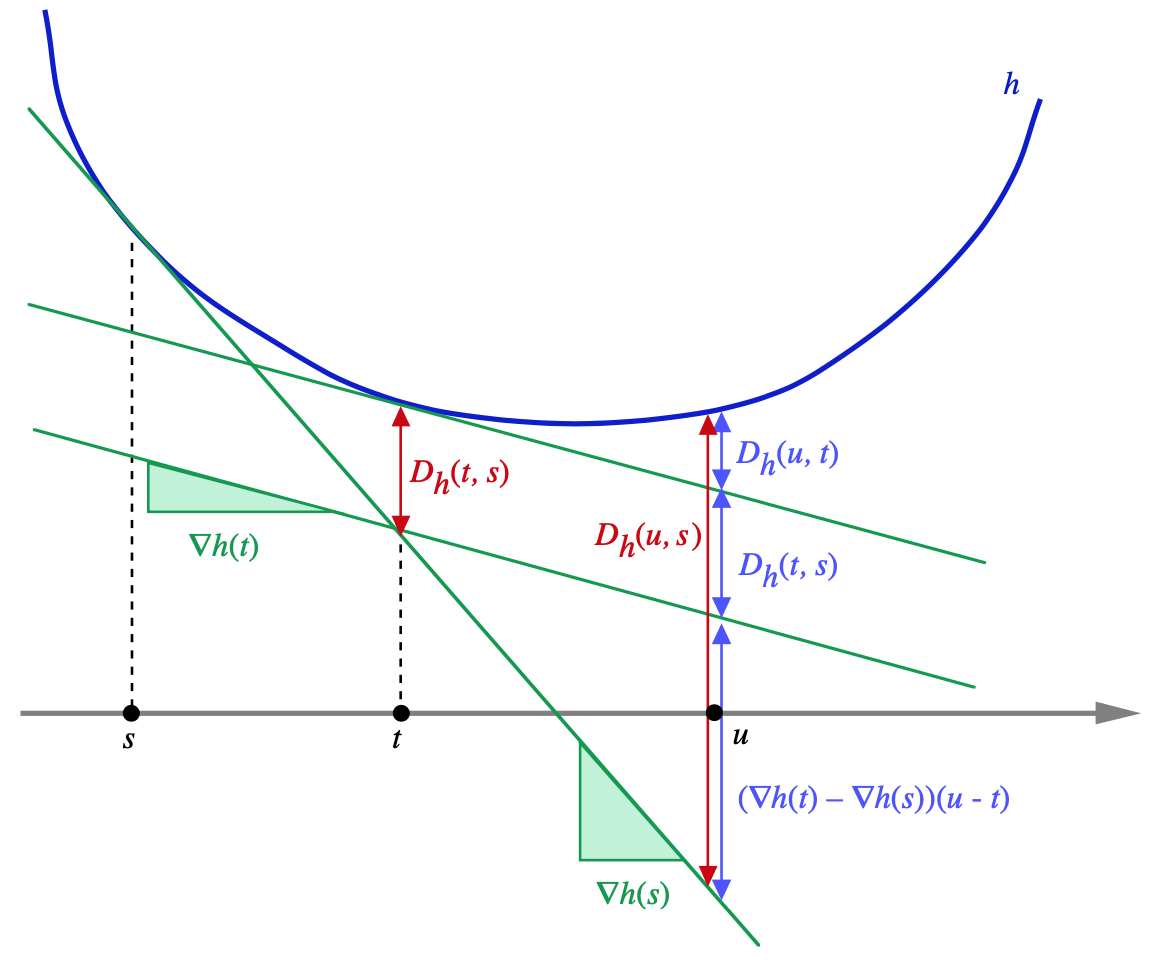
\includegraphics[width=.7\textwidth]{figs/3pointslemma}
	\caption{Illustration of the other three points lemma -- eg the identity between Bregmans -- taken from \citet{eckstein1998approximate}.}
	\label{fig:3pointslemma}
\end{figure}

The typical descent lemma of updates involving minimization of a Bregman divergence is called the three point lemma. 
It corresponds to first order optimality conditions of the update.
With its hep, one can prove convergence for mirror descent with relative smoothness, or for Bregman proximal point algorithms.

\begin{lemma}
Let $x_+$ be a solution to 
\begin{align}
	x_+ \in \argmin	_{x\in C} \overbrace{f(x) + \cB_h(x ; y)}^{\phi(x)}
\end{align}
where $C$ is a closed convex set, $f$ is a convex function, $\cB_h$ is the Bregman divergence induce by some convex function $h$, and $y$ is some reference vector. Then 
\begin{align}
	\forall x, f(x) + \cB(x ;y) \geq f(x_+) + \cB(x ; x_+) +\cB(x_+ ; y) \; .
\end{align}
\end{lemma}

Taking an information geometry lens, this property is analog to the Pythagorean theorem for generalized projections.
We recover euclidean projections setting $f=0$ and $h=\|.\|^2$.

\begin{proof}
	The first order optimality condition is
	\begin{align}
		&\langle \nabla \phi (x_+) , x -  x_+ \rangle \geq 0, \forall x \\
		=& \langle \nabla f(x_+) + \nabla h(x_+) - \nabla h (y), x - x_+ \rangle  
	\end{align}
	This proof relies on another property called three point property 
	\begin{align}
		\langle \nabla h(x_+) - \nabla h (y), x - x_+ \rangle  =\cB(x;y) -\cB(x;x_+) - \cB(x_+;y) 
	\end{align}
	which can be proved by expanding the right hand side.
	By convexity of $f$ we also have 
	\begin{align}
		 f(x_+) + \langle \nabla f(x_+), x - x_+ \rangle \leq f(x) \; .
	\end{align} 
	Putting it all together we get
	\begin{align}
		0 
		&\leq  \langle \nabla f(x_+), x - x_+ \rangle + \langle \nabla h(x_+) - \nabla h (y), x - x_+ \rangle  \\
		&\leq f(x) - f(x_+) + \cB(x;y) -\cB(x;x_+) - \cB(x_+;y)
	\end{align}
	which concludes the proof.
\end{proof}


\section{Relative Smoothness for Mirror Descent}
In the classic setting, SMD is studied under strong-convexity assumption on the mirror map $\logpart$ \citep{bubeck2015convex}.
In our setting this is not always true -- eg gaussians.
However a recent and fast-expanding body of work is concerned with a new assumption: relative smoothness and relative strong-convexity.
\begin{align}
	& \text{$f$ is $L$-smooth relative to $h$} \\
	\iff & Lh - f \ \text{convex} \\
	\iff & f(y) \leq 	f(x) + \langle \nabla f(x) , y-x \rangle + L\cB_h(y;x), \forall x,y \\
	\iff & \cB_f(y;x) \leq L \cB_h(y;x), \forall x,y \\
	\iff & \nabla^2 f(x) \leq L \nabla^2 h(x),  \forall x
\end{align} 
where the last equivalence holds only when $f$ and $h$ are twice differentiable. In words, $f$ is upper bounded by it linear approximation plus the $h$-Bregman divergence, which can also be seen as a bound between divergences, or more locally as a bound between Hessians. Similarly, $f$ is $\mu$ strongly-convex relative to $h$ if
\begin{align}
	& f-\mu h \ \text{ convex} \\
	\iff & f(x) + \langle \nabla f(x) , y-x \rangle + \mu \cB_h(y;x) \leq f(y)\forall x,y \\
	\iff & \mu\cB_h(y;x) \leq \cB_f(y;x) \forall x,y \\
	\iff & \mu \nabla^2 h(x) \leq \nabla^2 f(x)  \forall x \; .
\end{align} 

Another way to view this elegant generalization of smoothness and strong-convexity is as a transfer of the Loewner partial order on symmetric matrices to functions, via the Hessian. 
As such it can be applied to many functions that were out of reach for $\ell^2$ norm, by taking the appropriate reference function.  For instance $h(x) = -\log(x)$ or $h(x) = x^4$. 
As early as 2011, \citet{birnbaum2011distributed} showed $O(\inv{t})$ convergence rate for mirror descent under smoothness assumption relative to the mirror map. 
More precisely, he proved that when $f$ is $L$-smooth relative to $h$, then the suboptimality of the sequence 
\begin{align}
	x_{t+1}  = \argmin_x \langle \nabla f(x_t), x \rangle + \cB_h(x ; x_t)
\end{align}
is upper bounded by the simple formula
\begin{align}
	\implies f(x_t) - f(x_*) \leq \frac{L \cB_h(x_* ; x_0) }{t} \; .
\end{align}
These notions were rediscovered and expanded by \citet{bauschke2017descent} and \citet{lu2018relatively}. If you need to read one, pick \citet{lu2018relatively} -- I found it much much easier and more enjoyable to read.  This latter paper also derived a linear convergence rate for mirror descent under relative smoothness and strong-convexity, with the relative condition number $\frac{L}{\mu}$ appearing.


\subsection{Convergence of Mirror Descent}
\paragraph{Descent Lemma.}
To get the descent lemma, apply successively relative smoothness, 3 points lemma, and relative strong convexity on $f$. Note that the strong convexity constant $m$ may be zero. Recall that $\ell_f(\natp, \natp^{t}) = f(\natp^t) + \langle \nabla f (\natp^t) ; \natp - \natp^t \rangle $ is the linearization of $f$ at $\natp^t$ evaluated in $\natp$. 
\begin{align}
	f(\natp^{t+1}) 
	&\leq \ell_f(\natp^{t+1}, \natp^{t})  + L \bregman(\natp^{t+1}; \natp^{t})
	& \text{(Relative $L$-smoothness)} \\
	& \leq \ell_f(\natp^{*}, \natp^{t})  + L \bregman(\natp^{*}; \natp^{t}) -L \bregman(\natp^{*}; \natp^{t+1}) 
	& \text{(3 Points Lemma w. $x=\natp^*$)} \\
	& \leq f(\natp^*) + (L - m) \bregman(\natp^{*}; \natp^{t}) -L \bregman(\natp^{*}; \natp^{t+1}) 
	& \text{(Relative $m$-strong convexity)}
\end{align}

\paragraph{Monotonicity.}
Applying the 3 points lemma with $x=\natp_t$, 
\begin{align}
	f(\natp^{t+1}) \leq  f(\natp^t) -L (\bregman(\natp^{t}, \natp^{t+1}) + \bregman(\natp^{t+1} , \natp^{t} ))
\end{align}
shows the function value is monotonically decreasing, and we the gap at each step is greater than the symmetrized bregman between iterates. 

\paragraph{No Strong-Convexity.}
The simpler case is when $m=0$, then we get a telescopic sum
\begin{align}
	\sum_{t=0}^{T-1} (f(\natp^{t+1}) - f(\natp^*)) 
	&\leq L \sum_t \bregman(\natp^{*}; \natp^{t}) - \bregman(\natp^{*}); \natp^{t+1}) \\
	&= L \bregman(\natp^{*}; \natp^{0}) - L\bregman(\natp^{*}); \natp^{T})\\
	&\leq L \bregman(\natp^{*}; \natp^{0}) \; ,
\end{align}
from which we can conclude thanks to the monotonicity of $f(\natp^t)$
\begin{align}
	f(\natp^{T}) - f(\natp^*)
	\leq  \frac{L}{T} \bregman(\natp^{*}; \natp^{0}) \; ,
\end{align}

\paragraph{Strong Convexity.} 
When $m>0$, we need to do some cooking with a coefficient $\frac{L-m}{L}$ to create the telescopic sum
\begin{align}
	\sum_{t=0}^{T-1} \left( \frac{L-m}{L} \right)^{T-1-t} (f(\natp^{t+1}) - f(\natp^*)) 
	&\leq \sum_{t=0}^{T-1} \frac{( L-m)^{T-t}}{L^{T-t -1}} \bregman(\natp^{*}; \natp^{t}) 
	- \frac{( L-m)^{T-t-1}}{L^{T-t-2}} \bregman(\natp^{*}); \natp^{t+1}) \\
	&= \frac{( L-m)^{T}}{L^{T-1}}  \bregman(\natp^{*}; \natp^{0}) 
	- L \bregman(\natp^{*}); \natp^{T}) \\
	&\leq L \left( \frac{L-m}{L} \right)^T \bregman(\natp^{*}; \natp^{0}) \; .
\end{align}
Then using the monotonicity of $f(\natp^t)$, we end up with the geometric sum of $\frac{L-m}{L} < 1$
\begin{align}
		\sum_{t=0}^{T-1} \left( \frac{L-m}{L} \right)^{T-1-t} (f(\natp^{t+1}) - f(\natp^*)) 
		&\geq (f(\natp^{T}) - f(\natp^*)) \sum_{t=0}^{T-1} \left( \frac{L-m}{L} \right)^{T-1-t} \\
		&\geq (f(\natp^{T}) - f(\natp^*)) \inv{1 - \frac{L-m}{L}} \\
		&= (f(\natp^{T}) - f(\natp^*)) \frac{L}{m} \; .
\end{align}
Finally we end up with the final iterate linear convergence rate
\begin{align}
	f(\natp^{T}) - f(\natp^*)
	\leq m  \left( 1 - \frac{m}{L} \right)^T \bregman(\natp^{*}; \natp^{0}) 
\end{align}
featuring $\frac{L}{m} $ the relative condition number.

\section{Cramer-Rao Lower Bound}
In statistics, there is this famous theorem known as the Cramer-Rao lower bound. In its simplest form, it states that the covariance of an unbiased estimator of a distribution's parameter $\natp$ is lower bounded by the inverse Fisher information matrix, divided by $n$
\begin{align}
    \Cov(\hat \natp_n)  
    &\succeq \inv{n} \cI(\natp_*)^{-1} \\
    \iff
    \expect[\cD\sim \natp_*]{(\hat \natp_n - \natp_*)(\hat \natp_n - \natp_*)^T}
    &\succeq \inv{n} \expect[X\sim \natp_*]{-\nabla^2 \log p(X|\natp_*)}^{-1} \; .
\end{align}
This is a typical statistic bound, which is concerned with the $\ell^2$ accuracy of an estimator, via its covariance. In contrast, here we are concerned with the quality of the estimator in terms of KL-divergence, eg "how accurately am I modeling this distribution?"

Note that in the case of an exponential family, the lower bound is always reached for the MLE estimator $\hat \mu_n$, because $\cI(\mu) = \nabla^2 \conj(\mu) = \nabla^2 \logpart(\natp)^{-1} = \Cov(T(X))^{-1}$, where the first step takes some calculus. For the estimator $\hat \natp_n$, this lower bound is not trivial.

In our case, the bias variance decomposition tells us that we are interested in the covariance between primal and dual parameters, rather than the covariance of only of these -- $\Cov(\MAPt;\MAPm)$ rather that $\Var(\MAPm)$ or $\Var(\MAPt)$.

\section{Posterior Expected Loss}

A conjugate prior for the exponential family with sufficient statistic $T(X)$ and natural parameter $\natp$ is written as
\begin{align}
    p(\natp) 
    \propto \exp(-n_0 \bregman(\natp ; \natp_0)) 
    \propto \exp(-n_0 \logpart(\natp) + \langle n_0 \mu_0 ; \natp \rangle) \; .
\end{align}
We see that $p(\natp)$ is part of the exponential family, with sufficient statistic $(\natp, \logpart(\natp))$ and natural parameters $(n_0 \mu_0 , -n_0)$. When we update this prior with Bayes formula on dataset $\cD=(x_1,\dots,x_n)$, we get a posterior $p(\natp | \cD)$ with natural parameters $(n_0 \mu_0 + \sum_i T(x_i) , -(n_0 + n))$. This is well detailed in \citet{agarwal2010geometric}. 

Given this posterior, a natural quantity to consider is the expected loss. Thus we might ask "what is the expectation of the posterior expected suboptimality?"
\begin{align}
    \expect[\cD\sim\natp_*]{\expect[p(\natp|\cD)]{\bregman(\natp ; \natp_*)}}
\end{align}
This quantity is even harder to estimate than the expected MAP suboptimality, because of the double integral. We can get a closed form for the age-old $\ell^2$ loss of $\cN(\mu, 1)$, which yields the exact rate $\inv{n}$. This is exactly twice the expected loss of the MLE.

\begin{example}
	We can also get a closed form for the posterior of a centered gaussian variance 
	\begin{align}
		\expect[p(\natp|\cD)]{\bregman(\natp ; \natp_*)} = \bregman(\hat \natp_n ; \natp_*) + \frac{2}{n} \frac{\mu_*}{\hat \mu_n} + \log\frac{n}{2} - \psi(1 + \frac{n}{2})
	\end{align}
	using the mean of the \href{https://en.wikipedia.org/wiki/Inverse-gamma_distribution}{inverse Gamma distribution} and the \href{https://en.wikipedia.org/wiki/Gamma_distribution#Logarithmic_expectation_and_variance}{logarithmic expectation} of a Gamma. 
	Then using results from the MLE, we get the exact formula
	\begin{align}
		\expect[\cD\sim\natp_*]{\expect[p(\natp|\cD)]{\bregman(\natp ; \natp_*)}}
		= \frac{2}{n} + \frac{2}{n(n-2)} + \psi(\half[n]) - \psi(1+ \half[n])
	\end{align}
	and we bound it to 
	\begin{align}
		\inv{2n} + \frac{4}{n(n-2)}
		\leq \expect[\cD\sim\natp_*]{\expect[p(\natp|\cD)]{\bregman(\natp ; \natp_*)}}
		\leq 
		\inv{n} + \frac{4}{n(n-2)}
	\end{align}
	which is about twice the MLE bounds~\eqref{eq:MLE_rate}, exactly as we reportred for the gaussian mean.
\end{example}


\section{Gaussian Variance}
\subsection{Proof of MLE Tight Bound}
	\begin{theorem}[MLE tight upper bound]
	The MLE of $\cN(0,\mu_*)$ is $\mu_n = \inv{n} \sum_i X_i^2 $.
	Its expected suboptimality is infinite when $n\leq 2$ and otherwise
	\begin{align}
		 \expect{\bregmanconj( \mu_*; \mu_n) }
			\leq \inv{2n} +\frac{2}{n(n-2)} \; .
	\end{align}
	\end{theorem}
	
	\begin{proof}
	The ratio to the optimum  $\frac{\mu_n}{\mu_*}$follows a \href{https://en.wikipedia.org/wiki/Chi-square_distribution}{Chi-square distribution} with $n$ degrees of freedom $\chi^2(n)$ divided by $n$. Its inverse $\frac{\mu_*}{ \mu_n} $ follows an \href{https://en.wikipedia.org/wiki/Inverse-chi-squared_distribution}{inverse Chi-square distribution} with expectation 
	\begin{align}
		\expect{\frac{\mu_*}{ \mu_n}  - 1} 
		= \expect{\frac{n}{\chi^2(n)} - 1} =
		\begin{cases}
			\frac{n}{n-2} -1 = \frac{2}{n-2} \ \text{ if } n>2, \\
			+\infty \  \text{ otherwise. }
		\end{cases}
	\end{align}
	There is also a closed form solution for the expected logarithm of a Chi-squared\citep{pav2015moments}
	\begin{align}
		\expect{\log \frac{\mu_n}{\mu_*}} = \psi(\half[n]) - \log(\half[n])
	\end{align}
	where $\psi$ is the \href{https://en.wikipedia.org/wiki/Digamma_function}{digamma function.}
	Consequently the suboptimality of the MLE has a closed form solution
	\begin{align}
	\expect{\bregmanconj( \mu_*; \mu_n) }
	&= \half \expect{\frac{\mu_*}{ \mu_n} - 1 + \log \left(\frac{\mu_n}{\mu_*} \right) } \\
	& =
	\begin{cases}
		\half \left ( \frac{2}{n-2} +\psi(\half[n]) - \log(\half[n]) \right )  \ \text{ if } n>2, \\
			+\infty \  \text{ otherwise. }
	\end{cases}
	\end{align}
	It is surprising that we need more than $3$ samples for the loss to have a bounded expectation. 
	It is also very pleasant that the optimal value $\mu_*$ does not appear in this rate, so that the convergence rate is independent of the actual solution.
	When the expectation is finite, we can make its formula intelligible thanks to \href{https://en.wikipedia.org/wiki/Digamma_function#Inequalities}{bounds on the digamma function}
	\begin{align}
		-\inv{x} \leq \psi(x) - \log(x) \leq -\inv{2x}	\; .
	\end{align}
	  For $n\geq 3$,
	\begin{align}
		\inv{n-2} - \inv{n}
		&\leq \expect{\bregmanconj( \mu_*; \mu_n) }
		\leq \inv{n-2} - \inv{2 n} \\
		\iff
			\frac{2}{n(n-2)}
			&\leq \expect{\bregmanconj( \mu_*; \mu_n) }
			\leq \inv{2n} +\frac{2}{n(n-2)}
	\end{align}
	so we get a $O(n^{-2})$ lower bound and a $O(n^{-1}) + O(n^{-2})$ upper bound.
	\end{proof}
	Using the \href{https://en.wikipedia.org/wiki/Digamma_function#Recurrence_formula_and_characterization}{Stirling series}, we can also get an asymptotic approximation
	\begin{align}
		\expect{\bregmanconj( \mu_*; \mu_n) }
		\in \inv{2n} + \frac{11}{6 n^2} + \frac{4}{n^2(n-2)} + O(n^{-4}) \; .
	\end{align}
	
	
\subsection{Proof of MLE Loose Upper Bound}
If we apply \eqref{eq:log_bound} to the MLE, we get the upper bound
\begin{align}
	\expect{\bregmanconj(\mu^*; \MAPm^\text{MLE})}
	&\leq  \half \left( \expect{\frac{n}{\chi^2(n)}} + \expect{\frac{\chi^2(n)}{n}} - 2 \right ) \\
	&= \half \left( \frac{n}{n-2} + 1 - 2 \right)  
	= \frac{1}{n-2}
\end{align}
which is exactly  an additive term $1/2n$ larger than \eqref{eq:MLE_rate}. This highlights the factor $2$ difference between the log-bound and an exact computation of the expectation of the log term, and a tight upper bound on the digamma function.

\subsection{Multivariate MLE}
In higher dimensions $d$
 \begin{align}
 	\expect{\bregmanconj( \mu_*; \hat \mu_n^\text{MLE(d)})}
 	= \half \left ( \frac{d(d+1)}{n-d-1} + \psi_d(\half[n]) - d \log(\half[n])  \right )
 \end{align}
where $\psi_d(\half[n]) = \sum_{i=0}^{d-1} \psi ( \half[n - i])$ is the multivariate digamma function.
Using the same upper bound as in the univariate case
\begin{align}
	\psi_d(\half[n]) - d \log(\half[n]) 
	\leq \sum_{i=0}^{d-1} \log(1 - \frac{i}{n}) - \frac{1}{n-i} \; .
\end{align}
We can bound the harmonic sum with typical bounds
\begin{align}
	- \sum_{i=0}^{d-1} \frac{1}{n-i} 
	&= H_{n-d} - H_n \\
	&\leq \log(n-d) + \gamma + \inv{2(n-d) - 1} - \log(n) - \gamma - \inv{2n+1}\\
	&= \log(1-\frac{d}{n})  + \frac{2(d + 1)}{(2n+1)(2(n - d) - 1}
\end{align}
which yields 
\begin{align}
	\psi_d(\half[n]) - d \log(\half[n]) 
	\leq \sum_{i=0}^{\textcolor{red}{d}} \log(1 - \frac{i}{n})
	+ \frac{2(d + 1)}{(2n+1)(2(n - d) - 1}  \; .
\end{align}
From there we have two options. 
Either we use a concave tangent bound on the logarithms to get
\begin{align}
	\sum_{i=0}^{d} \log(1 - \frac{i}{n})
	\leq \sum_{i=0}^{d} - \frac{i}{n}
	 = -\frac{d(d+1)}{2n}
\end{align}
which yields the final rate
\begin{align}
 	\expect{\bregmanconj( \mu_*; \hat \mu_n^\text{MLE(d)})}
 	\leq \frac{d(d+1)}{4n} + \frac{d(d+1)^2 + \half[d+1]}{2 n (n - d -1)} \;.
\end{align}
Note that this rate is not tight for $d>1$, but it is tight for $d=1$, and we almost recover the previous rate.

Another option, potentially tighter than the tangent bound, is to bound the sum of logarithms with an integral, using the monotonicity of the logarithm $\log(1 - \frac{i}{n}) \leq \log(1- \frac{x}{n}) , \forall x \in [i - 1, i]$
\begin{align}
	\sum_{i=1}^{d} \log(1 - \frac{i}{n})
	&\leq \int_{0}^{d} \log(1- \frac{x}{n}) dx \\
	& = n \int_{1 - \frac{d}{n}}^{1} \log(y) dy \\
	& = n [ y (\log(y) - 1) ]_{1 - \frac{d}{n}}^{1} \\
	& =  - n - (n -d) (\log ( 1 - \frac{d}{n}) - 1) \\
	& = - (n -d) \log ( 1 - \frac{d}{n}) - d \; .
\end{align}
Unfortunately, it is hard to get a tractable and non-vacuous bound for this guy. At $n=d$ it is worth $-d$, and then it grows up to $0$. and we can bound it using some exponents of $1 - \frac{d}{n}$, but that is not really helpful to get an easy formula.
Actually looking at \href{https://www.desmos.com/calculator/q4sqk73tld}{graphics}, the first upper bound turns out to be tighter than the second one. 

\subsection{Proof of Expected MAP Natural Parameter}
Let us introduce a variable characterizing the importance of the prior
\begin{important}
	\begin{align}
			a=n_0 \frac{\mu_0}{\mu^*} \; .
	\end{align}
\end{important}
\begin{lemma}[Expected MAP natural parameter]
	The expectation of the natural parameter of the MAP of $\cN(0,\mu_*)$ is bounded as
\begin{equation}
		\frac{\mu^*}{\mu_n}
		\leq \expect{\frac{\mu^*}{\MAPm}} 
		= \expect{\frac{\MAPt}{\natp^*}} 
		\leq \begin{cases}
		\frac{n_0 +n}{a+n-2} \text{ when } n\geq 2,\\
		\frac{n_0 +1}{a} \text{ when } n=1.
		\end{cases}
		\label{eq:lemma_natp_bound}
	\end{equation}
\end{lemma}

\begin{proof}
	The lower bound can be readily obtained with the Jensen inequality applied on the convex function $x\mapsto\inv{x}$ for $x>0$.
	The upper bound requires much more work.
	To start, let us plug in the definition of $\MAPm$
	\begin{align}
		\expect{\frac{\mu^*}{\MAPm}} 
		= \expect{\frac{\MAPt}{\natp^*}} 
		&= \expect{\frac{(n_0+n) \mu^*}{n_0 \mu_0 + \sum_i X_i^2}}  \\
		&= (n_0 + n) \expect{\inv{n_0 \frac{\mu_0}{\mu^*}+ \sum_i \frac{X_i^2}{ \mu^*} }} \\
		&= (n_0 +n) \expect{\inv{a + \chi^2(n)}}
	\end{align}
	where $\chi^2(n) = \sum_i \frac{X_i^2}{ \mu^*}$ is a chi-square random variable of degree $n$ and $a=n_0 \frac{\mu_0}{\mu^*}$.
	We reformulate this expectation with the trick
	\begin{align}
		&\int_1^\infty e^{-\frac{zt}{2}} dt = \frac{2}{z} e^{-\half[z]} \\
		\implies &\inv{z} = \half e^{\half[z]} \int_1^\infty e^{-\frac{zt}{2}} dt \\
		\implies &\inv{a+x} = \half e^{\frac{a+x}{2}} \int_1^\infty e^{- \frac{(a+x)t}{2}}dt \; ,
	\end{align} 
	to get two integrals instead of one
	\begin{align}
		2^{\half[n]}\Gamma(\half[n]) \expect{\inv{a + \chi^2(n)}}  
		&= \int_0^\infty \frac{x^{\frac{n}{2}-1}e^{-\half[x]} }{a+x} dx \\
		&= \int_0^\infty dx\  x^{\frac{n}{2}-1}e^{-\half[x]} \half e^{\half[a+x]} \int_1^\infty  dt\  e^{-\half[(a+x)t]}  \\
		&= \half e^{\half[a]} \int_1^\infty dt \ e^{-\half[a t]}   \int_0^\infty dx \  x^{\frac{n}{2}-1} e^{-\half[x t]}  \; ,
	\end{align}
	where we used Fubini to switch integrals, without further justification.
	Now with the change of variable $x = 2\frac{y}{t}$, eg $dx = 2\frac{dy}{t}$, the inner integral becomes
	\begin{align}
		\expect{\inv{a + \chi^2(n)}}  
		&= \frac{e^{\half[a]} }{2^{\half[n]+1}\Gamma(\half[n]) }\int_1^\infty dt \ e^{-\half[a t]}   \int_0^\infty 2\frac{dy}{t} \  (2\frac{y}{t})^{\frac{n}{2}-1} e^{-y} \\
		&= \frac{e^{\half[a]} }{2\Gamma(\half[n]) } 
		\underbrace{\int_1^\infty  \frac{e^{-\half[a t]}}{t^{\frac{n}{2}}}  dt}_{E_{\half[n]}(\half[a])  } \ 
		\underbrace{\int_0^\infty  y^{\frac{n}{2}-1} e^{-y} dy}_{\Gamma(\half[n])}
	\end{align}
	so we finally get  the formula valid for all $n\geq 1$
	\begin{align}
		\boxed{\expect{\inv{a + \chi^2(n)}}  = \half e^{\frac{a}{2}} E_{\half[n]}(\half[a])}
		\label{eq:hard_expectation}
	\end{align}
	where the \href{https://dlmf.nist.gov/8.19}{generalized exponential integral function} is defined as 
	\begin{align}
		E_k(z) = \int_1^\infty \frac{e^{-z t} }{t^k} dt \; .
	\end{align}
	Now our goal is to bound this function with simpler functions.
	Fortunately, mathematicians have been working on these integrals for decades.
	When $n=2$, eg $k=1$, we have the simple exponential integral function which \href{https://dlmf.nist.gov/6.8.E1}{verifies the bound}
	\begin{align}
		\half \log(1 + \frac{2}{x}) 
		\leq e^x E_1(x) 
		\leq \log(1+\inv{x}) \leq \inv{x} \; .
	\end{align}
	For $n \geq 2$, eg $k\geq 1$, we have \href{https://dlmf.nist.gov/8.19.E21}{the general bound}
	\begin{align}
		\inv{x+k}
		\leq e^x E_k(x) 
		\leq \inv{x + k - 1}
	\end{align}
	so that 
	\begin{align}
		\inv{a+n}
		&\leq \expect{\inv{a + \chi^2(n)}}
		\leq \inv{a + n - 2} \\
		\iff \frac{n +n_0}{a + n}	
		&\leq  \expect{\frac{\mu^*}{\MAPm}} 
		\leq \frac{n +n_0}{a + n - 2}	\\
		\iff \frac{\mu^*}{\mu_n}
		&\leq \expect{\frac{\mu^*}{\MAPm}} 
		\leq \frac{1}{\frac{\mu_n}{\mu^*} - \frac{2}{n + n_0}}  
	\end{align}
	where we used $\frac{a + n}{n +n_0} = \frac{\mu_n}{\mu^*}$.
	
We are left with a special case when  $n=1$, eg $k=\half$. 
Then we can use the trivial bound 
\begin{align}
	\expect{\inv{a + X^2}} < \inv{a}
	\label{eq:trivial_bound}
\end{align}
which is what we are using in the lemma,
or we can get a stronger result with further derivations.
The integral can be written with \href{https://dlmf.nist.gov/7.8.E1}{Mill's ratio} $M(x) = e^{x^2} \int_x^\infty e^{-t^2} dt$, by doing the change of variable $t= x \sqrt{u}$, $dt=\frac{x}{2} \frac{du}{\sqrt{u}}$ 
\begin{align}
	& \int_x^\infty e^{-t^2} dt 
	= \frac{x}{2} \int_1^\infty \frac{e^{-x^2 u}}{\sqrt{u}} du 
	= \frac{x}{2} E_{\half}(x^2) \\
	\implies & M(x) = \frac{x}{2} e^{x^2} E_{\half}(x^2) \\
	\implies & e^{y} E_{\half}(y) = 2 \frac{M(\sqrt{y})}{\sqrt{y} }
\end{align}
so that 
\begin{align}
		\expect{\inv{a + X^2}} 
		= \half e^{\half[a]} E_{\half[1]}(\half[a]) 
		= \sqrt{\frac{2}{a}} M(\sqrt{\half[a]})
		= \frac{2}{a} \sqrt{\half[a]} M(\sqrt{\half[a]}) \; .
\end{align}
Then using \href{https://dlmf.nist.gov/7.8.E8}{another bound from the DLMF}, we get that 
\begin{align}
	\inv{a+1}
	\leq \expect{\inv{a + X^2}} 
	< \inv{a}\left( 1 - \inv{a+3} \right) \; .
\end{align}
\end{proof}


\subsection{Proof of MAP Bound}
\begin{theorem}[MAP Upper Bound]
 The expected suboptimality of the MAP of $\cN(0,\mu^*)$ with prior hyper-parameters $(n_0,\mu_0)$ is 
\begin{equation}
	\expect{\bregmanconj( \mu_*; \hat \mu_n^\text{MAP})}
	\leq \begin{cases}
		\bregmanconj( \mu_*; \mu_0) \ \text{ if } \ n=0, \\
		\inv{2(n_0+1)}  + \frac{(1 + \inv{n_0} - \frac{\mu_0}{\mu^*})^2}{2 \frac{\mu_0}{\mu^*}(1 + \inv{n_0} )} \ \text{if}\ n=1,\\
		\frac{1}{n_0 \frac{\mu_0}{\mu^*} +n-2} + \frac{(1 + \inv{n_0} - \frac{\mu_0}{\mu^*})^2}{2 (\frac{\mu_0}{\mu^*}+\frac{n-2}{n_0})(1 + \frac{n}{n_0} )} \ \text{if}\ n\geq 2
	\end{cases}
\end{equation}
\end{theorem} 

\begin{proof}
When $n=0$, the inequality is an equality. 
Wen $n>0$, Wolfram finds no closed form for $\expect{\log\frac{\MAPm}{\mu^*}}$ so we focus on the simple log-bound given by \eqref{eq:log_bound},
\begin{align}
	2\expect{\bregmanconj(\mu^*; \MAPm)} 
	&\leq \expect{\frac{\mu^*}{\MAPm}} -1  + \expect{\frac{\MAPm}{\mu^*}} - 1 \; .
\end{align}
We readily get 
\begin{align}
	 \expect{\frac{\MAPm}{\mu^*}} - 1 = \frac{a+n}{n_0+n} - 1 = \frac{a - n_0}{n_0+n}
\end{align}
where recall that $a=n_0\frac{\mu_0}{\mu^*}$. 
There remains the more problematic term with the expectation of the inverse mean parameter.
Fortunately, we derived the bound \eqref{eq:lemma_natp_bound} for this purpose.

\textbf{When $n\geq 2$}, we get 
\begin{align}
	\expect{\frac{\mu^*}{\MAPm}} - 1 
	\leq \frac{n_0 + n}{a +n - 2} -1
	= \frac{n_0 - a + 2}{a +n - 2}
	 = \frac{2}{a +n - 2} + \frac{n_0 - a}{a +n - 2}
\end{align}
so putting it all together we get 
\begin{align}
	\expect{\bregmanconj(\mu^*; \MAPm)} 
	&\leq \frac{1}{a+n-2} + \frac{n_0-a}{2}  \left( \inv{a+n-2} - \inv{n_0+n} \right)\\
	&\leq \frac{1}{a+n-2} + \frac{n_0-a}{2}  \frac{n_0 - a + 2}{(a+n-2)(n_0+n)} \\
	&= \frac{1}{a+n-2} + \frac{(n_0 - a)^2 + 2(n_0-a) \pm 1}{2(a+n-2)(n_0+n)} \\
	&= \frac{1}{a+n-2} + \frac{(n_0 - a +1)^2 - 1}{2(a+n-2)(n_0+n)} \\
	&\leq \frac{1}{a+n-2} + \frac{(n_0 - a +1)^2}{2(a+n-2)(n_0 + n)} \\
	&= \frac{1}{a+n-2} + \frac{(1 + \inv{n_0} - \frac{\mu_0}{\mu^*})^2}{2 (\frac{\mu_0}{\mu^*}+\frac{n-2}{n_0})(1 + \frac{n}{n_0} )} \; .
\end{align}

\textbf{When $n=1$} the bound~\eqref{eq:lemma_natp_bound}  on the expected natural parameter gives
\begin{align}
	\expect{\frac{\mu^*}{\MAPm}} - 1 
	\leq \frac{n_0 + 1}{a} -1
	= \frac{n_0 +1 - a}{a}
\end{align}
so putting it all together we get
\begin{align}
	2\expect{\bregmanconj(\mu^*; \hat \mu_1)} 
	&\leq \frac{a - n_0 \pm 1}{n_0 + 1}  + \frac{n_0 - a + 1}{a} \\
	& = \inv{n_0+1}  + ( a - n_0 - 1)(\inv{n_0+1} - \inv{a}) \\
	& = \inv{n_0+1}  + \frac{(n_0 + 1 -a)^2}{a(n_0+1)}\\
	&= \inv{n_0+1}  + \frac{(1 + \inv{n_0} - \frac{\mu_0}{\mu^*})^2}{2 \frac{\mu_0}{\mu^*}(1 + \inv{n_0} )} 
\end{align}
so we do recover the same bias variance structure as when $n\geq2$.
\end{proof}

\section{More on the Bias-Variance Decomposition}

\subsection{Bias Term}
The pure bias term measures the divergence between the optimum and the expected MAP estimate $\bregmanconj(\mu^*; \mu_n)$.

\paragraph{Asymptote.}
Using the quadratic approximation of the Bregman divergence near $\mu^*$, we get a $O(n^{-2})$ rate for the pure bias term
\begin{align}
	\bregmanconj(\mu^*; \mu_n) 
	= \frac{\norm{\mu^* -  \mu_0}^2_{\mSigma^{-1}}}{2(1 + \frac{n}{n_0})^{-2} } + O(n^{-3}) \; .
\end{align}

\begin{example}
We can use the classical lower bound on the logarithm to upper bound the pure bias term 
	\begin{align}
		\bregmanconj(\mu^*; \mu_n)
		 &= \frac{\mu^*}{\mu_n} -1  - \log \frac{\mu^*}{\mu_n}  \\
		 &\leq \frac{(\mu^*- \mu_n)^2}{2 \mu^* \mu_n} 
		 = \half ( \frac{\mu^*}{\mu_n} + \frac{\mu_n}{\mu^*	}) - 1 \\		 
		 & =  \half (\frac{n_0 + n}{a + n} -1 + \frac{a +n}{n_0+n} -1) \\
		 & =  \half (\frac{n_0 - a}{a+n} + \frac{a - n_0}{n_0 + n}) \\
		 & = \half[n_0-a] (\inv{a+n} - \inv{n_0+n}) \\
		 &= \half[n_0-a] \frac{n_0 + n - a- n}{(a+n)(n_0+n)} \\
		 &= \frac{(n_0-a)^2}{2(a+n)(n_0+n)}
	\end{align}
	which is a $O(n^{-2})$ term, worth $0$ when $n_0=a$, eg $\mu_0=\mu^*$, exactly as we expected.
\end{example}

\subsection{Variance Term}

\paragraph{Asymptote.}
Using a linear approximation of the mirror map, we get a $O(n^{-1})$ rate for the covariance
\begin{align}
	&\nabla \conj(\mu)  
	= \nabla \conj(\mu^*) + \nabla^2\conj(\mu^*)(\mu - \mu^*) + O(\norm{\mu - \mu^*}^2) \\
	\implies &\hat \natp_n 
	= \natp^* + \Sigma^{-1} (\hat \mu_n - \mu^*)  + O(\E[\norm{\hat \mu_n - \mu^*}^2]) \\
	\implies &\Cov(\hat \natp_n ; T(X) ) 
	= \inv{n+n_0} \E[ \norm{T(X) - \mu^*}^2_{\Sigma^{-1}}]   + O(n^{-2}) \\
	\implies &\Cov(\hat \natp_n ; T(X) ) 
	 = \frac{d}{n+n_0} + O(n^{-2}) \; .
\end{align}
Note that we lost a factor $\half$ compared to the straightforward asymptotic analysis~\eqref{eq:MAP_asymptote}, probably because of the Jensen upper bound.

\begin{example}
	For the gaussian variance MAP, the variance term is
		\begin{align}
			\Cov(\hat \natp_n ; \hat \mu_n )  
			= \E[\MAPt \MAPm] - \E[\MAPt] \E[\MAPm] 
			=  - \half - \E[\MAPt] \mu_n
	\end{align}
	where we used the fact that $\natp \mu = -\half$ for all valid pairs $(\natp, \mu)$. 
	Plugging-in \eqref{eq:theta_expectation_bound} yield
	\begin{align}
		-\half + \frac{\mu_n}{2 \mu_n}
		&\leq \Cov(\hat \natp_n ; \hat \mu_n ) 
		\leq -\half + \half \frac{a + n}{a + n - 2} \\
		\iff 0&\leq \Cov(\hat \natp_n ; \hat \mu_n ) 
		\leq \half \frac{a+n - (a + n -2)}{a + n - 2} \\
		\iff 0&\leq \Cov(\hat \natp_n ; \hat \mu_n ) 
		\leq \inv{a +n - 2}
	\end{align}
	which is exactly the kind of upper bounds we were looking for !
\end{example}

\subsection{Mixed Bias-Variance Term}
The mixed bias variance term is $ \frac{n_0}{n+n_0} \langle  {\mu_* - \mu_0} ; {\natp_n - \E[\hat \natp_n]} \rangle $.
Note that it might be negative !
Let's focus on the right factor
\begin{align}
\theta_n - \expect{\hat \theta_n} = \nabla \conj(\E[\hat \mu_n]) - \E[\nabla \conj(\hat \mu_n)]
\end{align}
is sort of a commuting bracket between $\nabla \conj$ and the expectation over $\hat \mu_n$. It will be large if $\nabla \conj$ is highly non linear over the distribution of $\hat \mu_n$.

\paragraph{Asymptote.}
A linear approximation of $\nabla \conj$ shows that the mixed term is in $O(n^{-3})$, since the linear function commutes with the expectation.
We need to use a quadratic approximation of $\nabla \conj$ to get a non-trivial approximation
\begin{align}
	&\nabla \conj(\mu)  
	= \nabla \conj(\mu^*) + \nabla^2\conj(\mu^*)(\mu - \mu^*) +  \half \nabla^3 \conj(\mu^*) [ (\mu - \mu^*)  ; (\mu - \mu^*) ]
	+ O(\norm{\mu - \mu^*}^3) \\
	&\implies 
	\nabla \conj(\E[\hat \mu_n]) - \E[\nabla \conj(\hat \mu_n)]
	= \half \nabla^3 \conj (\mu^*) \Cov(\hat \mu_n) 
	+ O(\E[\norm{\hat \mu_n - \mu^*}^3]) \\
	&\implies 
	\nabla \conj(\E[\hat \mu_n]) - \E[\nabla \conj(\hat \mu_n)]
	= \frac{\nabla^3 \conj (\mu^*) \Sigma}{2(n+n_0)^2} 
	+ O(n^{-3}) \\
\end{align}
where the axis of the tensor product between third derivative and vector / matrix are all kept implicit for simplicity.
Consequently the bias-variance term is 
\begin{align}
	\frac{n_0}{n+n_0} \langle  \bias{\mu^* - \mu_0} ; \variance{\natp_n - \E[\hat \natp_n]} \rangle
	 = \frac{n_0}{(n+n_0)^3} (\mu^* - \mu_0)^\top \nabla^3 \conj (\mu^*) \Sigma + O(n^{-4}) = O(n^{-3}) \; .
\end{align}

\begin{example}
	As we have the tight bounds \eqref{eq:theta_expectation_bound} for the expectation of the natural parameter of the MAP, we can bound above and below this mixed term
	\begin{align}
		0
		\leq \natp_n - \E[\MAPt]
		\leq \frac{n_0 +n}{2 \mu^*} \left ( \inv{a+n-2} - \inv{a+n} \right)
		 = \frac{n_0+n}{\mu^*(a+n)(a+n-2)}	 \in O(n^{-1}) \; .
	\end{align} 
	Remark how this asymptotic class differs from the $O(n^{-2})$ I expected. Is this bound less tight than I thought, or are my calculus wrong ? 
	Also remark that $\natp_n$ is always greater than $\E[\MAPt]$, which is a good sanity-check because $\nabla \conj(\mu) = - \inv{2\mu}$ is a concave function.

	The rate on the mixed term depends on the sign of $\mu^* - \mu_0 $
	\begin{align}
		\frac{n_0}{n+n_0} \langle  \mu^* - \mu_0 ; \natp_n - \E[\hat \natp_n] \rangle
		\leq \begin{cases}
			0 \ \text{ if } \ \mu^*\leq \mu_0, \\
			\frac{n_0 - a}{(a+n)(a+n-2)} \ \text{ otherwise.}
		\end{cases}
	\end{align}
\end{example}


\subsection{Putting it all together}
\begin{example}
\begin{align}
	\expect{\bregmanconj(\mu^* ; \hat \mu_n)} 
	\leq \bias{\frac{(n_0-a)^2}{2(a+n)(n_0+n)}}
	+ \frac{\max(n_0 - a , 0)}{(a+n)(a+n-2)}
	+ \variance{\frac{1}{a+n-2}}
\end{align}
\end{example}

\subsection{More Illustrations of the Bias-Variance Decomposition}
See Figure~\ref{app:fig:bias-variance-numerical}.

\begin{figure}[p]
	\centering
	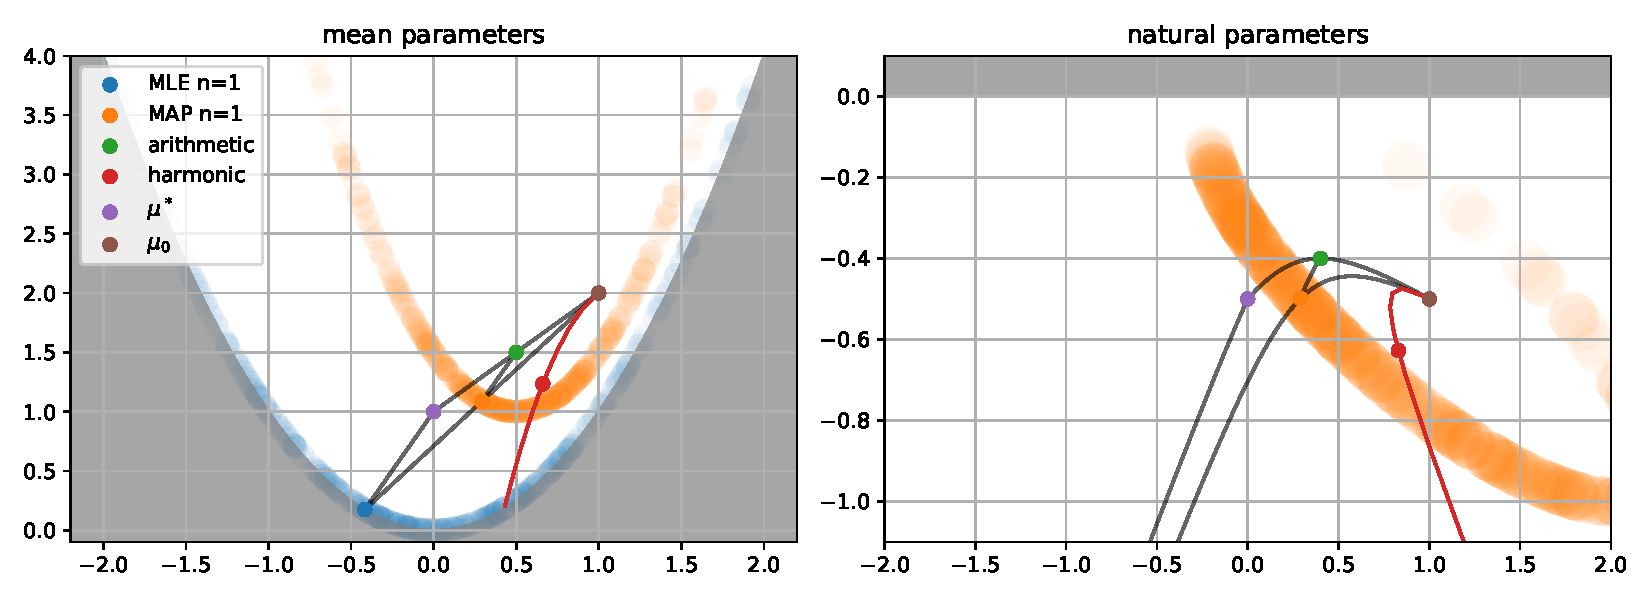
\includegraphics[width=\textwidth]{figs/thales/numerical_schema_n=1.pdf}
	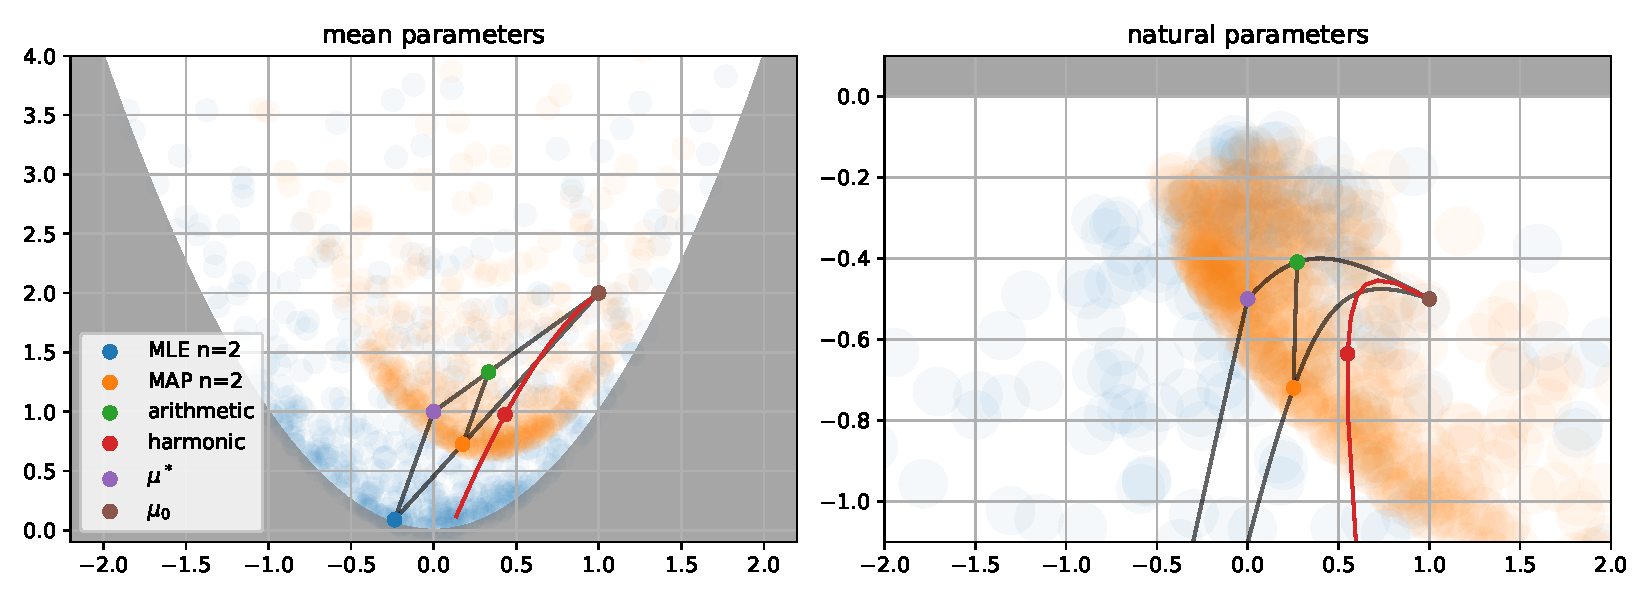
\includegraphics[width=\textwidth]{figs/thales/numerical_schema_n=2.pdf}
	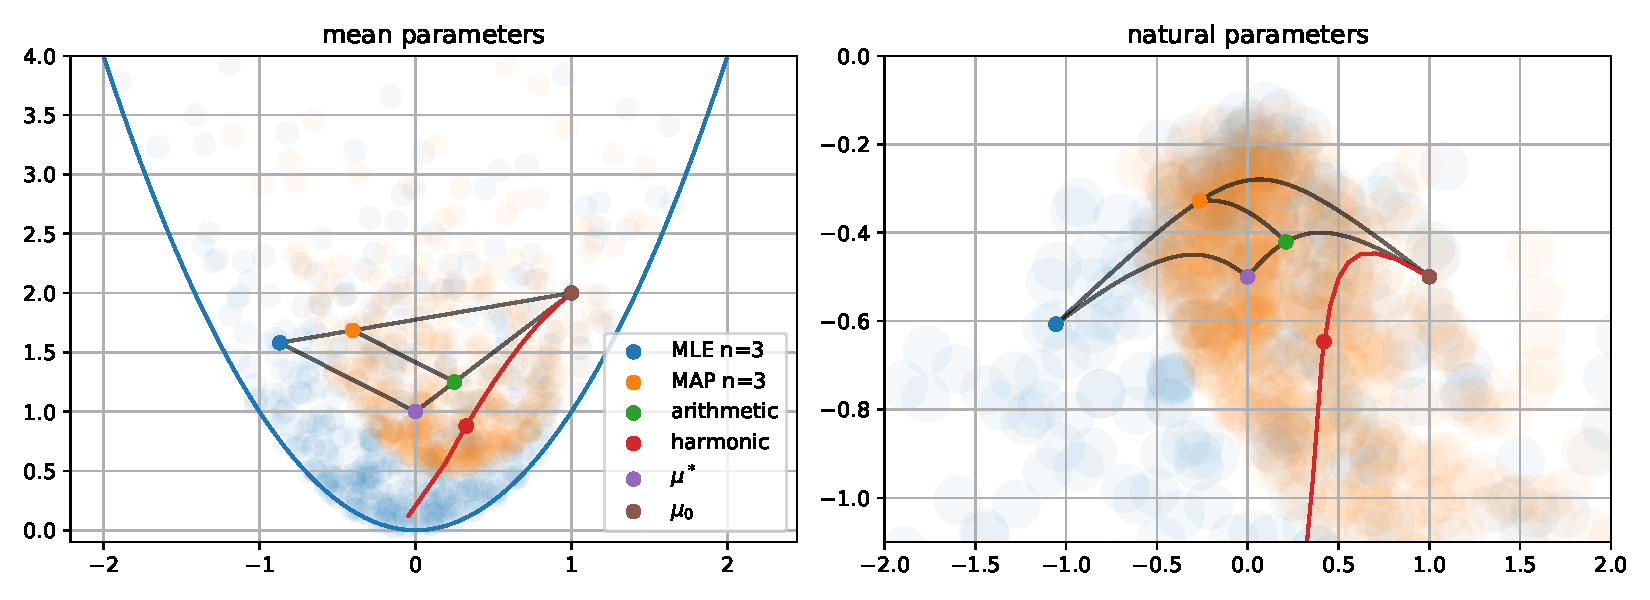
\includegraphics[width=\textwidth]{figs/thales/numerical_schema_n=3.pdf}
	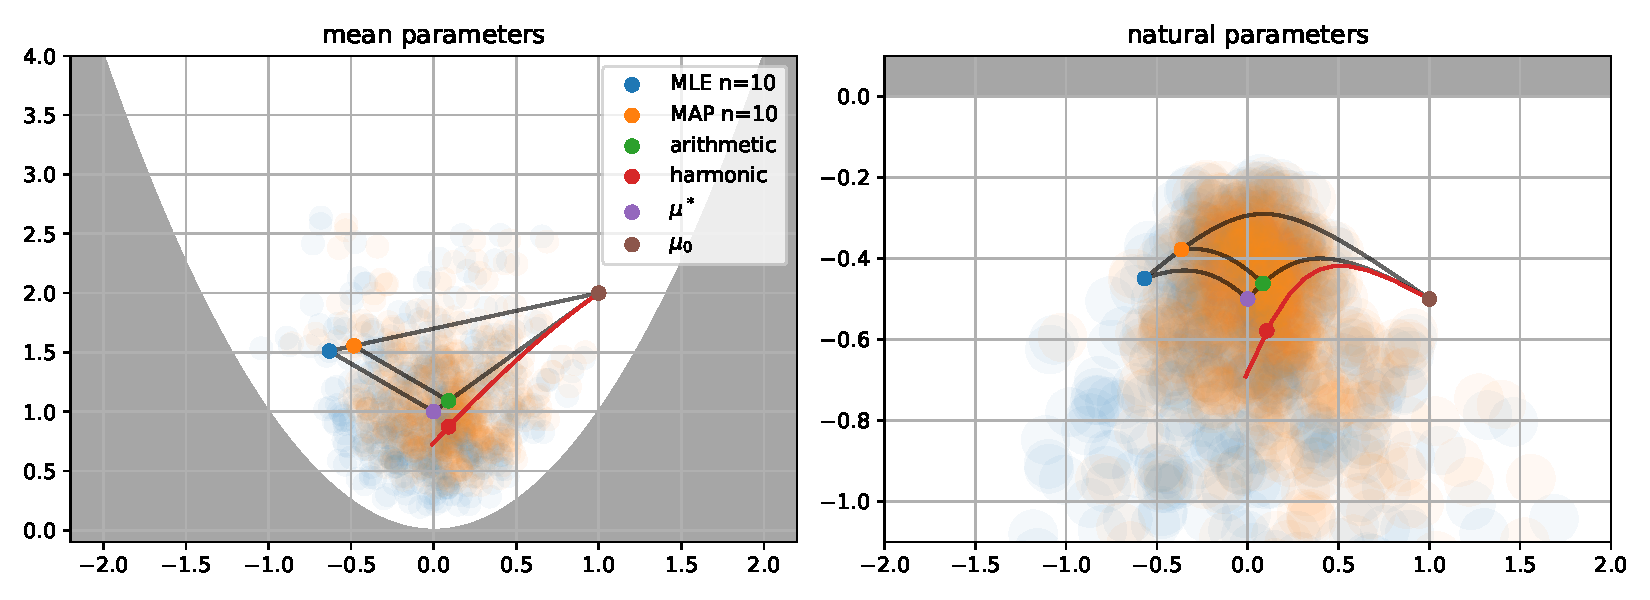
\includegraphics[width=\textwidth]{figs/thales/numerical_schema_n=10.pdf}
	\caption{A numerical illustration of the different characters featured in the bias-variance decomposition, for a 1D Gaussian $\cN(\mu, \sigma^2)$.}
	\label{app:fig:bias-variance-numerical}
\end{figure}

\clearpage

\section{Self-Concordance}
An hypothesis that may be more suitable than smoothness of Lipschitzness is self-concordance. $f: \real \rightarrow \real$ is self-concordant (SC) if 
\begin{align}
    \abs{f'''(x)} \leq 2 f''(x)^{\frac{3}{2}} \; .
\end{align}
The exponent $\frac{3}{2}$ is motivated by dimensional analysis and the factor $2$ appears to simplify downstream calculus.
A multidimensional function $f: \real^n \rightarrow \real$ is SC if it's restriction to any line is SC.
Most importantly, the negative logarithm $-\log(x)$ and its matrix generalization $-\log \det(\mX)$ (to verify) are self-concordant functions.
This is great, but it is missing all the other barrier objectives $x^{-\alpha}, \alpha>0$. 
For instance, gaussians have a logarithmic term, but hey also have an inverse term which is not self-concordant.
These other barriers can fit in the framework of  generalized self-concordance \citep{dvurechensky2020selfconcordant} , but the calculus quickly gets very complex, as this generalized self-concordance is not as clean as the standard self-concordance.

\paragraph{Questions.}
Is there already an SC analysis of proximal point methods. (that’s not affine invariant)?
If the log-partition is SC, then what does it mean for its gradient, the mapping from natural to mean parameters ? 

\subsection{Damien's Trials}

We want to have a rate of convergence on
\[
    \mathbb{E}_{X_i} \left[ \mathcal{B}_{A^*}(\mu_*,\mu_n) \right],
\]
where
\[
    \mu_* = \mathbb{E}_{X} T(X), \quad \mu_n =  \frac{\sum_{i=1}^n T(X_i) + n_0 \mu_0}{n_0+n}.
\]
We first assume that $A^*$ is self-concordant.

\paragraph{Notations}
\begin{itemize}
    \item $\|\cdot\|_x = \sqrt{ \langle \nabla^2A^*(x)\cdot,\, \cdot \rangle }$
    \item $\|\cdot\|_x^*= \sqrt{ \langle [\nabla^2A^*(x)]^{-1}\cdot,\, \cdot \rangle }$
    \item $\lambda(x) = \|(A^*)'(x)\|_x^*$ (Newton decrements)
    \item $\omega = t-\ln (1+t)$
    \item $\omega^* = -t-\ln(1-t)$
\end{itemize}
Note that $\omega^*$ is convex and monotonne.

\begin{proposition}
    (Conversion of norms) We have
    \[
        \frac{\|y-x\|_x}{1+\|y-x\|_x} \leq \|y-x\|_y \leq \frac{\|y-x\|_x}{1-\|y-x\|_x}
    \]
\end{proposition}


\begin{proposition}
    (Bounded Hessian change) We have
    \[
        (1-\|y-x\|_x)^2 \nabla^2 A^*(x) \leq \nabla^2 A^*(y) \leq \frac{1}{(1-\|y-x\|_x)^2} \nabla^2 A^*(x)
    \]
\end{proposition}


\begin{proposition}
    (Function bound) We have, if $\|y-x\|_x < 1$,
    \[
        A^*(y) \leq A^*(x) + \nabla A^*(x)(y-x) + \omega^*(\|y-x\|_x)
    \]
\end{proposition}

The last proposition implies that, when $\|y-x\|_x < 1$,
\[
    \mathcal{B}_{A^*}(y,x) \leq \omega^*(\|y-x\|_x).
\]
Therefore,
\[
    \mathcal{B}_{A^*}(\mu^*,\mu_n) \leq \omega^*(\|\mu^*-\mu_n\|_{\mu_n}) .
\]
then, if $\|\mu^*-\mu_n\|_{\mu^*} < 1$, we have
\[
    \mathcal{B}_{A^*}(\mu^*,\mu_n) \leq \omega^*\left(\frac{\|\mu^*-\mu_n\|_{\mu^*}}{1-\|\mu^*-\mu_n\|_{\mu^*}}\right) .
\]
Assume $\|\mu^*-\mu_n\|_{\mu^*} < c$,
\[
    \mathcal{B}_{A^*}(\mu^*,\mu_n) \leq \omega^*\left(\frac{\|\mu^*-\mu_n\|_{\mu^*}}{1-c}\right) .
\]

\paragraph{Discarded}
However,
\begin{align*}
    \|\mu^*-\mu_n\|^2_{\mu_n} & = \left\|\frac{n+n_0-1}{n+n_0}(\mu^*-\mu_{n-1}) + \frac{1}{n+n_0}(\mu^*-T_n)\right\|^2_{\mu_n},\\
    & = \left\|\frac{n+n_0-1}{n+n_0}(\mu^*-\mu_{n-1})\right\|_{\mu_n}^2 +  \left\|\frac{1}{n+n_0}(\mu^*-T_n)\right\|^2_{\mu_n} + \frac{2(n+n_0+1)}{(n+n_0)^2}\langle \nabla^2 [A(\mu_n)](\mu^*-\mu_{n-1}),\,(\mu^*-T_n) \rangle,\\
\end{align*}
and
\begin{align*}
    \|\mu^*-\mu_n\|_{\mu_n} & \leq  \frac{n+n_0-1}{n+n_0}\left\|\mu^*-\mu_{n-1}\right\|_{\mu_n} + \frac{1}{n+n_0}\left\|\mu^*-T_n\right\|_{\mu_n} .
\end{align*}
Moreover, by the bounded Hessian change,
\[
    \left\|\mu^*-\mu_{n-1}\right\|_{\mu_n} \leq \frac{1}{1-\left\|\mu_n-\mu_{n-1}\right\|_{\mu_{n-1}}}\left\|\mu^*-\mu_{n-1}\right\|_{\mu_{n-1}}
\]
    

\end{document}
